% !TeX encoding = UTF-8
% !TeX spellcheck = en_GB
% !TeX root = mythesis.tex


\chapter{Electron wavefunctions tomography}

In the previous chapter, we presented a new experimental method to investigate the charge properties of the elementary excitations in the quantum Hall effect.
This experimental study gives informations on the nature of the particles describing the excitations.
It also opens the way to other properties measurements with this technique in particular in the fractional quantum Hall effect.
In the integer quantum Hall effect the result is well established, the excitations are carried by electrons in the edge-channel.
Several effects from the manipulation of these electrons have been demonstrated, such as electronic Mach-Zehnder \cite{ji2003electronic,roulleau2007finite,litvin2007decoherence}, the Hanbury-Brown and Twiss experiment \cite{parmentier2010short,bocquillon2012electron,henny1999fermionic,oliver1999hanbury}, the Hong-Ou-Mandel interference \cite{bocquillon2013}, charge fractionalization \cite{bocquillon2013separation,freulon2015hong,hashisaka2017waveform,inoue2014charge}, energy relaxation \cite{le2010energy,marguerite2016decoherence,rodriguez2019strong,krahenmann2019auger}.
In this regime, the electronic excitations are now experimentally investigated at the level of the quantum state \cite{jullien2014quantum,marguerite2017extracting,santin2017quantum,fletcher2019quantum,freise2019full}.
In this chapter we measure the wavefunctions describing electron and hole excitations with different parameters.
The excitations are based on Lorentzian pulses carrying integer charges.
They are called Leviton from the reference \cite{levitov1996electro} which demonstrates that it is the pulse shape avoiding the emission of unwanted electron hole pairs.
The object chosen to represent these wavefunctions is the Wigner distribution.
The Wigner distribution is widely used for bosonic systems \cite{smithey1993measurement,lvovsky2009continuous,haroche2006exploring}.
%It is also introduced for electrons \cite{ferraro2013wigner}.
It has recently been introduced to describe electronic systems as well \cite{ferraro2013wigner}.
%And the measurement protocol used has been introduced theoretically \cite{grenier2011single}, and used experimentally \cite{marguerite2017two}.
Our experimental work follows the theoretical proposal of \cite{grenier2011single} and implemented experimentally for the first time in \cite{marguerite2017two}.
This chapter presents electronic wavefunctions and Wigner distributions, how they are linked and how we measure them, and discusses the results of measurements.

\section{\texorpdfstring{Wigner distribution and electronic wavefunctions}{Wigner distribution and electronic wavefunctions} \label{sec: Wigner distribution and electronic wavefunctions}}

\subsection{Description in terms of wavefunctions of a 1D system}

\subsubsection*{The wavefunctions in a quantum Hall edge-channel.}

In the integer quantum Hall effect regime, the edge channels are ballistic chiral 1D conductors.
An electron propagating along this conductor in a pure state is described by a wavefunction $\phi\left(x,t\right)$, with $x$ the position along the 1D conductor, and $t$ the time evolution.
In our case we will study a train of electrons emitted with a period $T$.
To begin with a simple situation of one electron in one state, we will consider a large enough period $T$ in order that the emissions from one period to the other are independent.
In this situation, the following paragraph details the informations carried by the electrical current and the occupation number.
They provide only partial informations on the wavefunction, hence the need for a time and energy representation with the Wigner distribution.
%In our case we always look at one fixed position chosen as $x=0$.
%This position is the quantum point contact location.
%So the electron wavefunction can be expressed only thanks to its time variable $\phi\left(t\right)$.
%A basic information we can deduce from this wavefunction is for example the probability $P_{\left[t_{1}; t_{2}\right]} $, given by \eqref{eq: probability presence}, of finding this electron between the time $t_{1}$ and $t_{2}$. 
A basic information we can deduce from this wavefunction is for example the probability $P_{\left[x_{1}; x_{2}\right]} $, given by \eqref{eq: probability presence}, of finding this electron between the positions $x_{1}$ and $x_{2}$ at a time $t_{0}$. 

%\begin{equation}
%P_{\left[t_{1}; t_{2}\right]} = \int_{t_{1}}^{t_{2}}|\phi\left(t\right)|^{2}\mathrm{d}t \label{eq: probability presence}
%\end{equation}

\begin{equation}
P_{\left[x_{1}; x_{2}\right]} = \int_{x_{1}}^{x_{2}}|\phi\left(x,t_{0}\right)|^{2}\mathrm{d}x \label{eq: probability presence}
\end{equation}

%The fermionic field operator $\hat{\Psi}^{\dagger}\left(t\right)$ enables to describe the state of an electron created at a time $t$.
%This state $\left|t\right>$ is the fermionic field operator applied on the vacuum $\left|\emptyset\right>$ \eqref{eq: time resolved state}.
In the experiment presented in the next section \ref{sec: Experimental determination of Wigner distribution}, the electronic system is observed in one fixed position chosen as $x=0$.
This position is the location of the quantum point contact used for the measurement of the wavefunction.
As the 1D conductor is modelled as ballistic and chiral, the wavefunction propagates from the position $x = 0$ with a speed which is equal to the Fermi velocity $v_{\mathrm{F}}$.
So the chosen description of a wavefunction as a function of time coordinate $t$ is equivalent to the description of the wavefunction in function of position $x$ at a fixed time.
The state of one electron created at a position $x$ is then replaced by an electron created at a time $t$ in equation \eqref{eq: time resolved state}.

%\begin{equation}
%\left|t\right> = \hat{\Psi}^{\dagger}\left(t\right)\left|\emptyset\right> \label{eq: time resolved state}
%\end{equation}

\begin{equation}
\left|t\right> = \sqrt{v_{\mathrm{F}}}\left|x = v_{\mathrm{F}}t\right> \label{eq: time resolved state}
\end{equation}

Similarly the wavefunction of an electron is expressed as a function of time by equation \eqref{eq: wavefunction in function of time}.

\begin{equation}
\left|\mathrm{e}\right> = \int_{-\infty}^{+\infty} \mathrm{d}x \phi\left(x,t_{0}\right)\left|x\right> = \int_{-\infty}^{+\infty} \mathrm{d}t \phi\left(t\right)\left|t\right> \Rightarrow \phi\left(t\right) = \sqrt{v_{\mathrm{F}}}\phi\left(x,t_{0}\right) \label{eq: wavefunction in function of time}
\end{equation}

%We also describe the state $\left|E\right>$ of an electron created at an energy $E$ with an operator $c^{\dagger}\left(E\right)$ linked to the fermionic field by the Fourier transform \eqref{eq: energy resolved state}.
We also describe the state $\left|E\right>$ of an electron created at an energy $E$ by the Fourier transform \eqref{eq: energy resolved state} of the state $\left|t\right>$.

%\begin{equation}
%\left|E\right> = c^{\dagger}\left(E\right)\left|\emptyset\right> = \frac{1}{\sqrt{h}}\int_{-\infty}^{+\infty}  e^{i\frac{Et}{\hbar}}\left|t\right>\mathrm{d}t = \frac{1}{\sqrt{h}}\int_{-\infty}^{+\infty}   e^{i\frac{Et}{\hbar}}\hat{\Psi}^{\dagger}\left(t\right)\left|\emptyset\right>\mathrm{d}t \label{eq: energy resolved state}
%\end{equation}
\begin{equation}
\left|E\right> = \frac{1}{\sqrt{h}}\int_{-\infty}^{+\infty}  e^{i\frac{Et}{\hbar}}\left|t\right>\mathrm{d}t \label{eq: energy resolved state}
\end{equation}

%The wavefunction of this state is expressed in function of time with the overlap \eqref{eq: wavefunction energy resolved state}. 
An electron wavefunction is expressed in function of energy with \eqref{eq: wavefunction energy resolved state}. 

%\begin{equation}
%\left<t^{\prime}\left|\right.E\right> = \frac{1}{\sqrt{h}}e^{i\frac{Et^{\prime}}{\hbar}} \label{eq: wavefunction energy resolved state}
%\end{equation}
\begin{equation}
\phi\left(E\right) = \int_{-\infty}^{+\infty} \mathrm{d}t \frac{1}{\sqrt{h}}e^{-i\frac{Et}{\hbar}}\phi\left(t\right) \label{eq: wavefunction energy resolved state}
\end{equation}

%With these two basis of states, $\left|t\right>$ and $\left|E\right>$, we can have an energy or a time representation of the electron pure state.
With these two basis of states, $\left|t\right>$ and $\left|E\right>$, we can have an energy or a time representation of the electron state.
These two representations are related to physical quantities which are the electrical current and the occupation.
The current is the number of electrons at position $x=0$ during a time $\mathrm{d}t$.
%So in the case of one pure electronic state it is the square modulus of the wavefunction in the time basis \eqref{eq: current pure state}.
So it is the square modulus of the wavefunction in the time basis \eqref{eq: current pure state}.

\begin{equation}
i\left(t\right) = -e \frac{\mathrm{d}}{\mathrm{d}t}\left(P_{\left[0;t\right]}\right) = -e|\phi\left(t\right)|^{2} \label{eq: current pure state}
\end{equation}

The occupation is the number of electrons at position $x=0$ in an energy interval $\mathrm{d}E$ during a period $T$.
Similarly to the current it is the square modulus of the wavefunction in the energy basis \eqref{eq: occupation pure state}.

\begin{equation}
f\left(E\right) = h\nu\frac{\mathrm{d}}{\mathrm{d}E}\left(P_{\left[0; E\right]}\right) = h\nu|\phi\left(E\right)|^{2} \label{eq: occupation pure state}
\end{equation}

with $\nu$ the fundamental frequency equals the inverse of the period $\nu = \frac{1}{T}$.

\subsubsection*{The time-energy representation.}

\begin{figure}[hptb]
	\begin{center}
			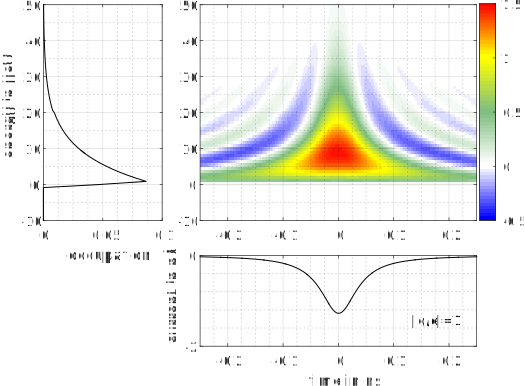
\includegraphics[width = 6.5cm]{./chap1/leviton_f_200MHz_tau_80ps_1microK_1e}
	\end{center}
	\caption{\textbf{Wigner distribution of a Leviton wavefunction carrying one electron.} The central colour plot is the Wigner distribution as a function of time as x-axis and energy as y-axis. The side graphs are current, below, and occupation, left. The current, obtained by integrated over the vertical energy axis, is a Lorentzian function, and the occupation, by integration over the horizontal time axis, is a decreasing exponential.}
	\label{fig: Wigner Leviton}
\end{figure}

%From the wavefunction in function of time $\phi\left(t\right)$ we access easily the time aspects of the electronic pure state, and we can measure them from the current.
From the wavefunction as a function of time $\phi\left(t\right)$, we access the time aspects of the electronic state easily, and we can measure them from the current.
But energy features are encoded in the phase of the wavefunction $\phi\left(t\right)$ and the current does not give information on them.
In the same way, we invert time and energy with the wavefunction as a function of energy $\phi\left(E\right)$ and the measurement of the occupation $f\left(E\right)$.
This leads to the analogue conclusion.
But we can also define a representation which gives access to both time and energy aspects, the Wigner distribution $W_{\phi}\left(E,t\right)$.
%It is a time-frequency representation used in physics \cite{wigner1997on,haroche2006exploring} but also in signal processing \cite{ville1948theorie,flandrin1998time,mallat1999wavelet}.
%This function is a two variables energy and time function.
%For a pure state $\phi$ it takes the following form \eqref{eq: wigner pure state}.
This distribution is a two variables energy and time function, which takes the following form \eqref{eq: wigner pure state} for a wavefunction $\phi$.
It is used in different domains: in physics \cite{wigner1997on,haroche2006exploring}, but also in signal processing \cite{ville1948theorie,flandrin1998time,mallat1999wavelet}.

%\begin{equation}
%W_{\phi}\left(E,t\right) = \int_{-\infty}^{+\infty} \phi^{\ast}\left(t+\frac{\tau}{2}\right)\phi\left(t-\frac{\tau}{2}\right) e^{-i\frac{E\tau}{\hbar}} d\tau = \int_{-\infty}^{+\infty} \phi^{\ast}\left(E+\frac{\epsilon}{2}\right)\phi\left(E-\frac{\epsilon}{2}\right) e^{-i\frac{\epsilon t}{\hbar}} d\epsilon \label{eq: wigner pure state}
%\end{equation}
\begin{equation}
W_{\phi}\left(E,t\right) = \int_{-\infty}^{+\infty} \phi^{\ast}\left(t+\frac{\tau}{2}\right)\phi\left(t-\frac{\tau}{2}\right) e^{-i\frac{E\tau}{\hbar}} d\tau \label{eq: wigner pure state}
\end{equation}

%It is a real function that displays the complete information on the pure state.
It is a real function that displays the complete information on the state.
Such as the wavefunction, but it is easier to interpret since there is no information encoded in the phase.
From the Wigner distribution, one can recover the current by integrating over energy at a fixed time $t$ \eqref{eq: time marginals wigner pure state}.
One can also recover the occupation during a period $T$ by integrating over time at fixed energy $E$ \eqref{eq: energy marginals wigner pure state}.

\begin{equation}
i\left(t\right) = -\frac{e}{h}\int_{-\infty}^{+\infty} W_{\phi}\left(E,t\right)\mathrm{d}E  \label{eq: time marginals wigner pure state}
\end{equation}

\begin{equation}
f\left(E\right) = \frac{1}{T}\int_{0}^{T} W_{\phi}\left(E,t\right)\mathrm{d}t \label{eq: energy marginals wigner pure state}
\end{equation}

When we plot the Wigner distribution with the time as x-axis and the energy as y-axis, time basis wavefunctions $\left|t\right>$ are vertical lines at fixed time $t$, and energy basis wavefunctions $\left|E\right>$ are horizontal lines at fixed energy $E$.
These lines correspond to the integration domain of current and occupation.
In the figure Fig. \ref{fig: Wigner Leviton}, the example of a Lorentzian wavefunction carrying a single electron, so called Leviton, is plotted following the above choice of axis.
The square moduli of the wavefunction in both basis are the current, which is a Lorentzian function whose integral is equal to one elementary charge, and the occupation, which is a decreasing exponential taking non-zero values above the Fermi level (taken as the energy reference). 
The Wigner distribution includes these both informations, as well as informations on the phase of the wavefunction.
The phase of the wavefunction manifests itself as fringes in the Wigner distribution and enables us to go beyond pure state analysis by studying mixed states as discussed in the next paragraph.

\subsubsection*{An electron in a mixed state.}

In addition to pure state like the above basis state, the electron can be in a mixed state.
The density matrix \cite{cahill1999density} describes these electronic states.
For a pure state, it is the density matrix of the corresponding wavefunction $\rho = \left|\phi\left>\right<\phi\right|$.
But there can be a statistical probability $p_{1}$ that the state is $\left|\phi_{1}\right>$ and  $p_{2}$ that the state is $\left|\phi_{2}\right>$.
In that case the total density matrix is $\rho = p_{1}\left|\phi_{1}\left>\right<\phi_{1}\right|+p_{2}\left|\phi_{2}\left>\right<\phi_{2}\right|$.
It is a different state than the coherent superposition of the two pure state $\left|\phi\right> = \sqrt{p_1}\left|\phi_1\right>+e^{i\theta}\sqrt{p_2}\left|\phi_2\right> $.
By extending the definition of the Wigner distribution to any density matrix with \eqref{eq: wigner density matrix}, it is possible to study the difference between pure and mixed state.

%\begin{equation}
%W_{\rho}\left(E,t\right) = \int_{-\infty}^{+\infty} \mathrm{Tr}\left(\hat{\Psi}^{\dag}\left(t+\frac{\tau}{2}\right)\rho\hat{\Psi}\left(t-\frac{\tau}{2}\right)\right)e^{-i\frac{E\tau}{\hbar}}d\tau \label{eq: wigner desity matrix}
%\end{equation}
\begin{equation}
W_{\rho}\left(E,t\right) = \int_{-\infty}^{+\infty} \left<t+\frac{\tau}{2}\right|\rho\left|t-\frac{\tau}{2}\right>e^{-i\frac{E\tau}{\hbar}}d\tau \label{eq: wigner density matrix}
\end{equation}

The Wigner distribution for a mixed state is just the weighted sum of the ones for each state $W_{\rho} = p_{1} W_{\rho_{1}}+p_{2} W_{\rho_{2}}$, whereas the Wigner distribution of a superposition shows an additional interference term $W_{\phi_{1}\phi_{2}}$ defined in \eqref{eq: Wigner coherent superposition}.

\begin{align}
W_{\rho} =&  p_{1} W_{\phi_{1}}+p_{2} W_{\phi_{2}} + 2\sqrt{p_{1}p_{2}}\Re\left(e^{i\theta}W_{\phi_{1}\phi_{2}}\right)\\ & \mathrm{with} \; W_{\phi_{1}\phi_{2}}=\int_{-\infty}^{+\infty} \phi_{2}^{\ast}\left(t+\frac{\tau}{2}\right)\phi_{1}\left(t-\frac{\tau}{2}\right) e^{-i\frac{E\tau}{\hbar}} d\tau \label{eq: Wigner coherent superposition}
\end{align}

These interferences induced by the last term of \eqref{eq: Wigner coherent superposition} are the signature that the Wigner distribution represents one pure wavefunction.
They appear as negative values or values above one.
For a classical state, we have a mixed state of a lot of wavefunctions and so all interference effects due to a coherent superposition are suppressed.
This implies that Wigner distribution is bounded between 0 and 1 for a classical state, like for example the measurement in \cite{fletcher2019quantum}.
So it can be interpreted classically as a probability distribution of finding an electron at a defined energy and time.
For a non-classical state the Wigner distribution does not respect these bounds, see figure Fig. \ref{fig: Wigner Leviton}, it is a quasi-probability distribution function.
It implies in the non-classical case that a time and an energy resolved measurement cannot be performed simultaneously.
%But if we performed a time resolved measurement we find the current.
%And if we performed an energy resolved measurement we find the occupation.
%The time and energy marginals correspond to these measurement, they are the overlap of the Wigner distribution with the Wigner distribution of an energy or time basis state.
%The equations for the marginals \eqref{eq: time marginals wigner pure state} and \eqref{eq: energy marginals wigner pure state} are true for the general case by replacing the pure state $\phi$ with the density matrix $\rho$.
The probability distributions, which may be correctly defined, are the marginals.
Marginals are the integral of the Wigner distribution along one axis, so they are the current and occupation given by equations \eqref{eq: time marginals wigner pure state} and \eqref{eq: energy marginals wigner pure state} with the density matrix $\rho$ replacing the wavefunction $\phi$.
The current marginal is the probability distribution given by a time resolved measurement, since its expression is also the overlap with a time basis state $\left|t\left>\right<t\right|$.
In the same way, the occupation marginal is the probability distribution given by an energy resolved measurement, since it is the overlap with an energy basis state $\left|E\left>\right<E\right|$.

\subsection{First order coherence of a many-body state.}

\subsubsection*{The Wigner distribution in the electronic case.}

Up to this point, all Wigner distribution properties are similar as the one for photons \cite{haroche2006exploring}.
But in 1D electronic conductors there are several differences appearing \cite{ferraro2013wigner}.
This subsection makes them explicit and adapts the Wigner distribution to the electronic conductors.
First even if at zero temperature we do not excite the system, the system is not the vacuum $\left|\emptyset\right>$ but it is a Fermi sea $\left|\mathrm{F}_{0}\right>$.
%This reference state of a zero temperature Fermi sea is an N-particle state described by a Slater determinant of N wavefunctions \eqref{eq: wavefunction Fermi sea}. 
This reference state of a zero temperature Fermi sea is an N-particle state, so to describe a system with several particles the Fermionic field operator $\hat{\Psi}^{\dagger}\left(t\right)$ is introduced.
This operator creates an electron at a time $t$, so the previous time basis state is linked to this operator and the vacuum $\left|\emptyset\right>$ by \eqref{eq: def fermionic field}.

\begin{equation}
\left|t\right> = \hat{\Psi}^{\dagger}\left(t\right)\left|\emptyset\right> \label{eq: def fermionic field}
\end{equation}

The Fermi sea at zero temperature is characterized by all the energy levels occupied up to the Fermi energy chosen as the zero of energy.
So an operator $\hat{c}\left(E\right)$, which creates an electron at the energy $E$, is more convenient.
It is derived from the Fourier transform \eqref{eq: def de c(E)} of the Fermionic field.

\begin{equation}
\hat{c}^{\dagger}\left(E\right) = \frac{1}{\sqrt{h}}\int_{-\infty}^{+\infty}e^{i\frac{Et}{\hbar}}\hat{\Psi}^{\dagger}\left(t\right)\mathrm{d}t \label{eq: def de c(E)}
\end{equation}

The energy basis states introduced in previous subsection is then easily expressed by \eqref{eq: def energy state with c(E)}.

\begin{equation}
\left|E\right> = \hat{c}^{\dagger}\left(E\right)\left|\emptyset\right> \label{eq: def energy state with c(E)}
\end{equation}

The advantage of these operators is that an N-particle state is constructed by accumulating N operators.
The Slater determinant of N wavefunctions is then naturally obtained by the anti-commutation relation of the operators.
For example, the Fermi sea at zero temperature state is \eqref{eq: wavefunction Fermi sea}.

\begin{equation}
\left|\mathrm{F}_{0}\right> = \prod_{E < 0}^{}c^{\dagger}\left(E\right)\left|\emptyset\right> = \mathrm{det}\left(\left|\phi_{E_{1}}\right>,...,\left|\phi_{E_{N}}\right>\right)_{E_{i}<0} \label{eq: wavefunction Fermi sea}
\end{equation}

with the Fermi energy chosen as the zero of energy. Its density matrix is \eqref{eq: density matrix Fermi sea}.

\begin{equation}
\rho_{\mathrm{F}_{0}} = \left(\prod_{E<0}^{}c^{\dagger}\left(E\right)\right)\left|\emptyset\left>\right<\emptyset\right|\left(\prod_{E^{\prime}<0}^{}c\left(E^{\prime}\right)\right) \label{eq: density matrix Fermi sea}
\end{equation}

The Wigner distribution defined for this state \eqref{eq: wigner many-body density matrix} probes the first order coherence by including a single pair of creation/annihilation Fermionic field operators.

\begin{equation}
W_{\rho}\left(E,t\right) = \int_{-\infty}^{+\infty} \mathrm{Tr}\left(\hat{\Psi}^{\dag}\left(t+\frac{\tau}{2}\right)\rho\hat{\Psi}\left(t-\frac{\tau}{2}\right)\right)e^{-i\frac{E\tau}{\hbar}}d\tau \label{eq: wigner many-body density matrix}
\end{equation}

For the zero temperature Fermi sea, it is an Heaviside function $W(E,t) = H(-E)$ plotted in figure Fig.\ref{fig: Wigner Fermi sea} panel (b).
Above this Heaviside function, we can define an electron state \eqref{eq: electron state}.

\begin{equation}
\left|\mathrm{e}\right> = \int_{0}^{+\infty}\phi_{\mathrm{e}}\left(E\right)c^{\dagger}\left(E\right)\left|\mathrm{F}_{0}\right>\mathrm{d}E \label{eq: electron state}
\end{equation}

By digging this Heaviside function, we can define a hole state \eqref{eq: hole state}, which is a type of excitation absent from photonic systems.

\begin{equation}
\left|\mathrm{h}\right> = \int_{-\infty}^{0}\phi_{\mathrm{h}}\left(E\right)c\left(E\right)\left|\mathrm{F}_{0}\right>\mathrm{d}E \label{eq: hole state}
\end{equation}

The most common kind of excitation we can think of is the thermal excitation.
The thermal state is a mixed state between different number of particle states weighted by the Fermi distribution \eqref{eq: density matrix finite temperature state}.

\begin{equation}
\rho_{\mathrm{F}_{T}} = \bigotimes_{E}^{}\left(f_{\mathrm{F}_{T}}\left(E\right)c^{\dagger}\left(E\right)\left|\emptyset\left>\right<\emptyset\right|c(E)+\left(1-f_{\mathrm{F}_{T}}\left(E\right)\right)\left|\emptyset\left>\right<\emptyset\right|\right) \label{eq: density matrix finite temperature state}
\end{equation}

In this density matrix \eqref{eq: density matrix finite temperature state}, there are states with zero electrons such as $\left|\emptyset\left>\right<\emptyset\right|$, or one electron in mode of energy $\epsilon$, $c^{\dagger}(\epsilon)\left|\emptyset\left>\right<\emptyset\right|c(\epsilon)$, and so on.
%This is a big difference with photon systems where usually only one mode is studied and so there is no concept of mixted state between different number of mode states but only between different wavefunctions of the same mode.
This is a big difference with photon systems where usually only one mode is studied.
One mode in photon systems corresponds to a single energy $E$ of the equation \eqref{eq: density matrix finite temperature state}, so the tensor product $\bigotimes_{E}$ is absent.
The energy basis state $c^{\dagger}\left(E\right)\left|\emptyset\right>$ of equation \eqref{eq: density matrix finite temperature state} is an analogue to the Fock state $a^{\dagger}\left|0\right>$ for photons, with for photons the possibility to create state with more than one photon in one mode.
This implies that the Wigner distribution gives all the informations of the photon states, because they only need the definition \eqref{eq: wigner density matrix} which includes a single mode and several wavefunctions with all the couples of time basis states $\left|t+\frac{\tau}{2}\right>$,$\left|t-\frac{\tau}{2}\right>$.
In the case of electrons the Wigner distribution defined in \eqref{eq: wigner many-body density matrix} probes only first order coherence, so it misses information between different electronic modes.
%For example as explained above the difference between a mixed state of two wavefunctions $\rho = \frac{1}{2}\left|\phi_1\left>\right<\phi_1\right|+\frac{1}{2}\left|\phi_2\left>\right<\phi_2\right|$ and a coherent superposition of these two wavefunctions $\rho = \frac{1}{2}\left(\left|\phi_{1}\right>+\left|\phi_{2}\right>\right)\left(\left<\phi_{1}\right|+\left<\phi_{2}\right|\right)$ is shown in the Wigner distribution.

%The difference between the Slater determinant of two particles $\rho = \frac{1}{2}c^{\dagger}_{1}c^{\dagger}_{2}|0><0|c_{1}c_{2} = \frac{1}{2}det(|\phi_1>,|\phi_2>)det(<\phi_1|,<\phi_2|)$ and the mixted state of the sum of two one particle state $\rho = \frac{1}{2}c^{\dagger}_{1}|0><0|c_{1}+\frac{1}{2}c^{\dagger}_{2}|0><0|c_{2} = \frac{1}{2}|\phi_1><\phi_1|+\frac{1}{2}|\phi_2><\phi_2|$ is also shown. Because the population are one for the Slater determinant and one-half for the mixed state.

\subsubsection*{The limitations of the first order Wigner distribution.}

%But not the difference between the mixed state of two one particle state $\rho = \frac{1}{2}c^{\dagger}_{1}|0><0|c_{1}+\frac{1}{2}c^{\dagger}_{2}|0><0|c_{2} = \frac{1}{2}|\phi_1><\phi_1|+\frac{1}{2}|\phi_2><\phi_2|$ and the mixed state of a Slater determinant and the vacuum $\rho = \frac{1}{4}c^{\dagger}_{1}c^{\dagger}_{2}|0><0|c_{1}c_{2}+\frac{1}{2}|0><0| = \frac{1}{2}\mathrm{det}(|\phi_1>,|\phi_2>)\mathrm{det}(<\phi_1|,<\phi_2|)+\frac{1}{2}|0><0|$.

%But the above Wigner distribution cannot show second order coherences.
The correlation between two different electronic mode, which is the second order coherences, is not shown in the Wigner distribution.
%For example we can have a mixed state of two Slater determinants of two particles states \eqref{eq: density matrix mixed of 2 Slater determinant}.
First we can consider a mixed state of two Slater determinants of two particles states \eqref{eq: density matrix mixed of 2 Slater determinant}.

\begin{equation}
\rho = \frac{1}{2}c^{\dagger}_{1}c^{\dagger}_{2}\left|\emptyset\left>\right<\emptyset\right|c_{1}c_{2}+\frac{1}{2}c^{\dagger}_{3}c^{\dagger}_{4}\left|\emptyset\left>\right<\emptyset\right|c_{3}c_{4} \label{eq: density matrix mixed of 2 Slater determinant}
\end{equation}

%Or the state can be in a coherent superposition of these two Slater determinants \eqref{eq: density matrix superposition of 2 Slater determinant}.
Then we can consider a coherent superposition of these two Slater determinants \eqref{eq: density matrix superposition of 2 Slater determinant}.

\begin{equation}
\rho = \frac{1}{2}\left(c^{\dagger}_{1}c^{\dagger}_{2}+c^{\dagger}_{3}c^{\dagger}_{4}\right)\left|\emptyset\left>\right<\emptyset\right|\left(c_{1}c_{2}+c_{3}c_{4}\right) \label{eq: density matrix superposition of 2 Slater determinant}
\end{equation}

The difference between these two states is not probed by the Wigner distribution.
Indeed the different terms $\frac{1}{2}c^{\dagger}_{1}c^{\dagger}_{2}\left|\emptyset\left>\right<\emptyset\right|c_{3}c_{4}$ between them always gives zero contributions in equation \eqref{eq: wigner density matrix}.
To go beyond these limitations, we need to generate time or inter-edge channel entangled states, that would require, as a theoretical object, higher coherence order Wigner distribution \cite{thibierge2015coherence,cabart2018measurement} and other set-up to generate and measure them \cite{hofer2017on,chirolli2011time,thibierge2016two} than the one used in this manuscript.
In this work, we will not be affected by these limitations, given that we will study time-dependant voltages applied via an ohmic contact or a gate on an edge-channel.
A single particle description is indeed enough with these excitations.
%But the both time and energy representation of the Wigner distribution will be useful for the time-dependant voltages excitations, contrary to DC signals like the finite temperature Fermi sea, where only the Fermi-distribution is enough as shown in figure Fig.\ref{fig: Wigner Fermi sea} panel (a).

%For the case of the finite temperature Fermi sea, the Wigner distribution in figure Fig.\ref{fig: Wigner Fermi sea} panel (a) gives all the informations even if there are different particle number states present in the system.
%In fact as it is a DC signal, the Fermi-distribution is enough to describe it, there is no time dependence.
%In this manuscript we will study time-dependant voltages applied via an ohmic contact or a gate on an edge-channel, so the both time and energy Wigner distribution is useful to describe the state.
%But we do not generate time or inter-edge channel intricate states, that would require higher coherence order Wigner distribution \cite{thibierge2015coherence,cabart2018measurement} and other set-up to generate and measure them \cite{hofer2017on,chirolli2011time,thibierge2016two}.

\subsection{Interpretation and elucidation of wavefunctions in the Wigner distributions}

In the above subsection, the electronic Wigner distribution is introduced and it is explained why it is the relevant function to measure in this work.
The following explains how the electronic wavefunctions can be extracted from the Wigner distribution using a diagonalization algorithm developed by B. Roussel during his PhD thesis \cite{roussel2017autopsy}.
%The following explains how the wavefunctions cited at the beginning of the chapter are visible in this function, by first clarifying with examples the meaning of different coefficients in the Wigner distribution, and then presenting a diagonalization algorithm in the B. Roussel PhD \cite{roussel2017autopsy} to get numerically the wavefunctions containing the single-particle information.

\subsubsection*{The excess Wigner distribution.}

\begin{figure}[hptb]
	\begin{center}
		\begin{tabular}{c c c c}
			(a) & & (b) &\\
			& 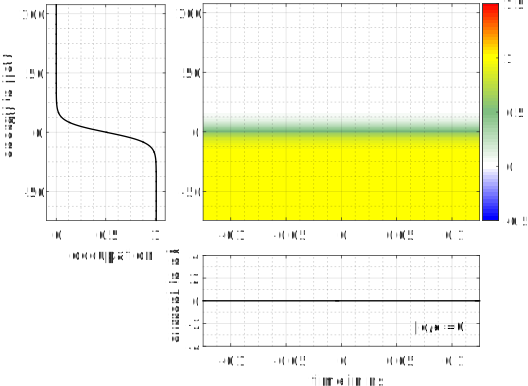
\includegraphics[width = 6.5cm]{./chap1/wig_finite_temp_fermi_sea}&
			& 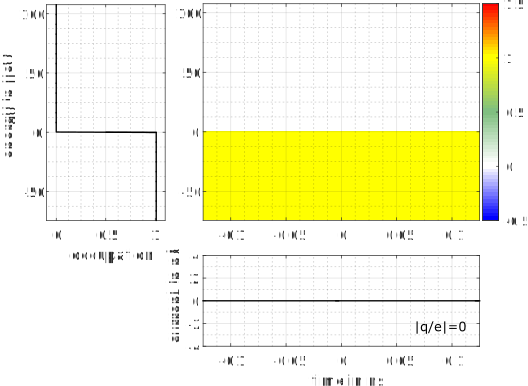
\includegraphics[width = 6.5cm]{./chap1/wig_zero_temp_fermi_sea} \\
			(c) & & & \\ 
			& 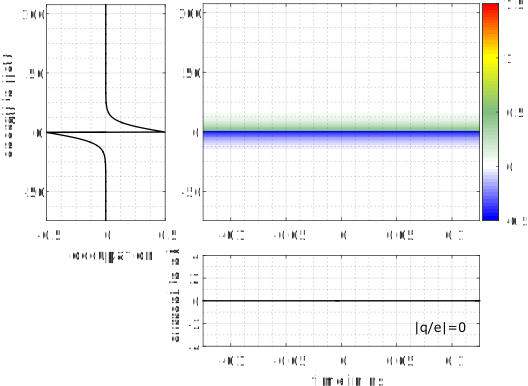
\includegraphics[width = 6.5cm]{./chap1/excess_wig_finite_temp_fermi_sea}&
		\end{tabular} 
	\end{center}
	\caption{\textbf{Wigner distribution of a finite temperature Fermi sea} \textbf{(a)} Wigner distribution of a Fermi sea at temperature $T_{\mathrm{elec}} = 51$ mK. The marginals are the occupation which is the Fermi distribution and the current which is the marginals of the excess Wigner distribution to be consistent with measurements. \textbf{(b)} Wigner distribution of the Fermi sea at zero temperature. Its occupation marginal is an Heaviside function, and as on the panel (a) the current is the marginal of the excess Wigner distribution. \textbf{(c)} Excess Wigner distribution of the Fermi sea of panel (a). It is calculated by subtracting Wigner distribution of panels (a) and (b), and shows thermal excitations.}
	\label{fig: Wigner Fermi sea}
\end{figure}

%From the electronic Wigner distribution measurement we extract all the single-particle informations.
The wavefunctions are excitations in addition to the reference state.
As the reference state is not the vacuum but a Fermi sea at zero temperature, we define the excess Wigner distribution \eqref{eq: definition excess Wigner} as the Wigner distribution from which we subtract the Wigner distribution of the reference state.

\begin{equation}
\Delta_{0}W(E,t) = W(E,t)-H(-E) \label{eq: definition excess Wigner}
\end{equation}

This excess Wigner distribution takes all excitations thermal and non-thermal into account.
We recover from the marginals of this excess Wigner distribution the measured electrical current $i\left(t\right)$, which is collected at a quantum point contact.
When no excitations are injected in the system, the current from the marginal of the excess Wigner distribution is the one equals zero.
From the other marginal, we recover the excess occupation of electrons and holes $\Delta_{0}f\left(E\right)$.
It shows holes occupation by negative values below the Fermi level.
The figure Fig. \ref{fig: Wigner Fermi sea} presents the example of a Fermi sea at finite temperature, with the Wigner distribution on the panel (a), the reference state Wigner distribution on the panel (b), and its excess Wigner distribution on the panel (c).

\subsubsection*{The electronic Glauber function.}

\begin{figure}[hptb]
	\begin{center}
		\begin{tabular}{c c c c}
			(a) & & (b) & \\
			
			& \includegraphics[height = 5cm]{./chap1/schema_Glauber}&
			& 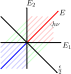
\includegraphics[height = 5cm]{./chap1/schema_Glauber_periodique}\\
			(c) &  & & \\ 
			& 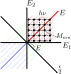
\includegraphics[height = 5cm]{./chap1/schema_Glauber_matrice}& &
		\end{tabular} 
	\end{center}
	\caption{\textbf{Schematics of the different coefficients of the energy coherence function.} \textbf{(a)} Illustration of the two energy variables $E_{1}$ and $E_{2}$ planes of the coherence function $\Delta_{0}G\left(E_{1},E_{2}\right)$. Red quadrant is about electronic properties, blue quadrant is for hole properties, and green quadrants are coherences between electron and holes. \textbf{(b)} Same illustration as for (a) in the specific case of a periodic excitation of fundamental frequency $\nu$. Only coefficients with the off-diagonal coordinate $\frac{\epsilon}{2}$ equals a multiple of $h\nu$ are different from zero. \textbf{(c)} Representation of coefficients involved in a matrix $M_{nm}$, defined in \eqref{eq: diagonalized matrix}, which links all electron states with possible coherence between them. These matrices for all $E$ between $0$ and $h\nu$ are diagonalized to find the wavefunctions emitted in the excitation.}
	\label{fig: schema Glauber}
\end{figure}


To evidence single-particle information, the excess Wigner distribution is converted to the energy coherence function by the Fourier transform along time \eqref{eq: definition Glauber function}.

\begin{equation}
\Delta_{0}G\left(E+\frac{\epsilon}{2},E-\frac{\epsilon}{2}\right) = \frac{1}{h}\int_{-\infty}^{+\infty} e^{i\frac{\epsilon t}{\hbar}}\Delta_{0}W\left(E,t\right) \mathrm{d}t \label{eq: definition Glauber function}
\end{equation}

This coherence function, called the electronic Glauber function \cite{grenier2011electron,haack2013glauber}, has the same information as the Wigner distribution but displays it in an energy-energy matrix form.
We identify different sectors in this energy-energy matrix.
The diagonal part of positive energies $\Delta_{0}G(E,E)$ with $E>0$, the red line in figure Fig.\ref{fig: schema Glauber} (a), is the probability to measure an electron at energy $E$, so it is the occupation $f(E)$.
The diagonal part of negative energies $E<0$, the blue line in Fig.\ref{fig: schema Glauber} (a), is the probability to measure a hole at energy $E$, so it is also the hole occupation as $f(E)-1$.
The off diagonal parts correspond to coherence terms between different energy states.
The positive quadrant is the sector where both arguments $E_1 = E+\frac{\epsilon}{2}$, $E_2 = E-\frac{\epsilon}{2}$ are positive.
It is the light red part of Fig.\ref{fig: schema Glauber} (a).
At this place the terms $\Delta_{0}G(E_1,E_2)$ correspond to a coherent superposition between the two electronic states $E_1$ and $E_2$.
In light blue, the coherent superpositions between holes fill the negative quadrant.
Finally, the green parts are superpositions of electrons and holes.

\subsubsection*{Glauber function examples of one electron.}

\begin{figure}[hptb]
	\begin{center}
		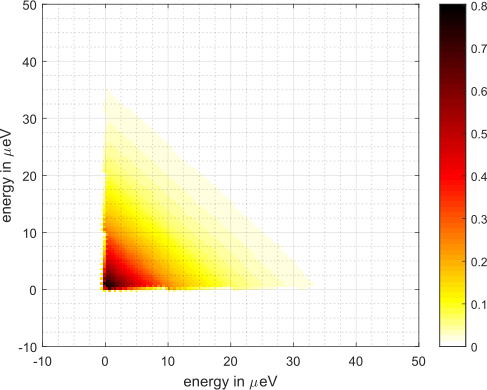
\includegraphics[width = 6.5cm]{./chap1/glauber_leviton_f_200MHz_tau_80ps_1microK_1e}
	\end{center}
	\caption{\textbf{Glauber function of a Leviton wavefunction carrying one electron.} The colour axis is the value of the Glauber function in ($\upmu$eV)$^{-1}$, plotted as a function of energy axis. It is computed from the Wigner distribution plotted in figure Fig. \ref{fig: Wigner Leviton} of a state with a Lorentzian wavefunction. The exponential decrease with the energy and the coherences for only positive energies shows that it is a pure electron state.}
	\label{fig: Glauber Leviton}
\end{figure}

We can take some examples of electronic states to illustrate information in the $\Delta_{0}G\left(E_{1},E_{2}\right)$ terms.
First we can have a statistical mixture between the state of energy $E_{1}$ and nothing given by \eqref{eq: mixed E_1 and nothing}.

\begin{equation}
\rho = \Delta_{0}G\left(E_1,E_1\right)c^{\dagger}\left(E_{1}\right)\left|\mathrm{F}_{T=0}\left>\right<\mathrm{F}_{T=0}\right|c\left(E_{1}\right)+\left(1-\Delta_{0}G\left(E_{1},E_{1}\right)\right)\left|\mathrm{F}_{T=0}\left>\right<\mathrm{F}_{T=0}\right| \label{eq: mixed E_1 and nothing}
\end{equation}

With this example $0 < \Delta_{0}G\left(E_{1},E_{1}\right) \leq 1$ and there is no population in other $E_{2}$ positive energy state $\Delta_{0}G\left(E_{2},E_{2}\right) = 0$, as shown in figure Fig. \ref{fig: schema Glauber examples} (a).
Since there is no population, there are no coherences either $\Delta_{0}G\left(E_{1},E_{2}\right) = 0$.
Another example is a coherent superposition of two energy state $E_{1}$ and $E_{2}$ like \eqref{eq: coherent superposition}.

\begin{equation}
\rho = \frac{1}{2}\left(c^{\dagger}\left(E_{1}\right)+c^{\dagger}\left(E_{2}\right)\right)\left|\mathrm{F}_{T=0}\left>\right<\mathrm{F}_{T=0}\right|\left(c\left(E_{1}\right)+c\left(E_{2}\right)\right) \label{eq: coherent superposition}
\end{equation}

It is deduced that the occupation and coherence terms are all equals $G(E_1,E_1) = G(E_2,E_2) = G(E_1,E_2) = G(E_2,E_1) = \frac{1}{2}$ like in figure Fig. \ref{fig: schema Glauber examples} (b).

With these two examples, we can interpret all the single electron cases.
So we can come back to the Leviton pure state used as an example in figure Fig. \ref{fig: Wigner Leviton}, and compute its Glauber function in figure Fig. \ref{fig: Glauber Leviton}.
For a pure state its expression \eqref{eq: Glauber pure state} is the product of the wavefunction at different energies.

\begin{equation}
\Delta_{0}G\left(E_1,E_2\right) = \phi\left(E_{1}\right)^{\ast}\phi\left(E_{2}\right) \label{eq: Glauber pure state}
\end{equation}

The diagonal on figure Fig. \ref{fig: Glauber Leviton} is exponentially decreasing as the occupation, and the coherences in the off-diagonal parts show the state is a pure state as the coherent superposition of energy states.
It also occupies only the electron quadrant, because it is a single electron state and there are no holes present.

\subsubsection*{Glauber function examples of several particles.}

The following examples concern examples with more than one electron, with two energy states simultaneously occupied and with an electron-hole pair.
With two electrons we can have a mixed state between a Slater determinant of the 2 particle state $E_1$ and $E_2$, the single particle state $E_1$ and $E_2$, and the vacuum, like for the Fermi sea \eqref{eq: mixed two particle states}.

%\begin{equation}
%\rho = \frac{1}{4}\left(1+c^{\dagger}\left(E_{1}\right)\right)\left(1+c^{\dagger}\left(E_{2}\right)\right)\left|\mathrm{F}_{T=0}\left>\right<\mathrm{F}_{T=0}\right|\left(1+c\left(E_{1}\right)\right)\left(1+c\left(E_{2}\right)\right) \label{eq: mixed two particle states}
%\end{equation}

\begin{align}
\rho =  &\frac{1}{4}\left|\mathrm{F}_{T=0}\left>\right<\mathrm{F}_{T=0}\right|\\
 + &\frac{1}{4}c^{\dagger}\left(E_{1}\right)\left|\mathrm{F}_{T=0}\left>\right<\mathrm{F}_{T=0}\right|c\left(E_{1}\right) +\frac{1}{4} c^{\dagger}\left(E_{2}\right)\left|\mathrm{F}_{T=0}\left>\right<\mathrm{F}_{T=0}\right|c\left(E_{2}\right) \\
 + &\frac{1}{4}c^{\dagger}\left(E_{1}\right)c^{\dagger}\left(E_{2}\right)\left|\mathrm{F}_{T=0}\left>\right<\mathrm{F}_{T=0}\right|c\left(E_{1}\right)c\left(E_{2}\right) \label{eq: mixed two particle states}
\end{align}

This example gives only diagonal terms $G(E_1,E_1) = G(E_2,E_2) = \frac{1}{2}$ and no off-diagonal terms $G(E_1,E_2) = G(E_2,E_1) = 0$.
This is represented in the panel (c) of figure Fig. \ref{fig: schema Glauber examples}.
Other proportions between the two particles mixed state and the one particle mixed state of this example have also the same terms.
This is due to the limitation at the first order coherence of the Wigner distribution studied.
For the specific example of a Slater determinant of two electrons as a pure state \eqref{eq : Slater determinant}, we can deduce information on the two particle state. 

\begin{equation}
\rho = \frac{1}{2}c^{\dagger}\left(E_{1}\right)c^{\dagger}\left(E_{2}\right)\left|\mathrm{F}_{T=0}\left>\right<\mathrm{F}_{T=0}\right|c\left(E_{1}\right)c\left(E_{2}\right) \label{eq : Slater determinant}
\end{equation}

Here we have fully populated states $E_{1}$ and $E_{2}$ with $G(E_1,E_1) = G(E_2,E_2) = 1$ and no coherence terms.
%For the negative quadrant, in blue in figure Fig.\ref{fig: schema Glauber} (a), when both arguments $E_1$, $E_2$ are negatives, we can have the same discussion with holes instead to electrons.
%The two last quadrants in green in Fig.\ref{fig: schema Glauber} (a), where $E_1$ and $E_2$ have different signs, are coherence between electrons and holes.
The last terms are coherences between electrons and holes.
%These terms are present for example with a superposition of an electron-hole pair and nothing expressed in equation \eqref{eq: electron/hole superposition} and drawn in figure \ref{fig: schema Glauber examples} (d).
These terms are present for example with a superposition of an electron at $E_{1}$ and a hole at $E_{2}$ pair, and nothing expressed in equation \eqref{eq: electron/hole superposition} and drawn in the figure \ref{fig: schema Glauber examples} (d).

\begin{equation}
\rho = \frac{1}{2}\left(1+c^{\dagger}\left(E_{1}\right)c\left(E_{2}\right)\right)\left|\mathrm{F}_{T=0}\left>\right<\mathrm{F}_{T=0}\right|\left(1+c\left(E_{1}\right)c^{\dagger}\left(E_{2}\right)\right) \label{eq: electron/hole superposition}
\end{equation}

\begin{figure}[hptb]
	\begin{center}
		\begin{tabular}{c c c c}
			(a) & & (b) & \\
			& 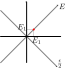
\includegraphics[height = 4cm]{./chap1/schema_Glauber_one_elec_state}&
			& \includegraphics[height = 4cm]{./chap1/schema_Glauber_superpos_two_elec} 
			\\
			(c) &  & (d) & \\ 
			& \includegraphics[height = 4cm]{./chap1/schema_Glauber_mixed_two_elec} &
			& \includegraphics[height = 4cm]{./chap1/schema_Glauber_matrice_superpos_elec_ho}
		\end{tabular} 
	\end{center}
	\caption{\textbf{Energy coherence function schematics of different state examples.} \textbf{(a)} The red point indicates the coordinates of the non zero values taken by the state of equation \eqref{eq: mixed E_1 and nothing}. \textbf{(b)} In this panel the state of equation \eqref{eq: coherent superposition} is studied. The state is a superposition of states at energies $E_{1}$ and $E_{2}$ and it has off-diagonal elements. \textbf{(c)} This panel correspond to the states of the two equations \eqref{eq: mixed two particle states} and \eqref{eq : Slater determinant}. If the diagonal values of the coherence function are below 1 the state can be in a mixed state between different particle number state. \textbf{(d)} The equation \eqref{eq: electron/hole superposition} defines a superposition between an electron hole pair and nothing. It has coherence term in electron hole quadrant shows in green.}
	\label{fig: schema Glauber examples}
\end{figure}

\subsubsection*{The diagonalization.}

With the examples, from chosen states we have computed values of the Glauber function.
The inverse problem of finding the states from the Glauber function has been developed and numerically implemented in the B. Roussel PhD manuscript \cite{roussel2017autopsy} and the article \cite{marguerite2017extracting}.
From the discussion above, we remark that the coherence function $\Delta_{0}G$ can be interpreted as a matrix, where diagonal elements are populations and off-diagonal elements are coherences.
In fact, there are two matrices, one for electrons, in the positive quadrant, and one for holes in the negative quadrant.
These two are diagonalized separately, to find the electronic wavefunctions and the hole wavefunctions present in the system.
%This diagonalization has been developped and numerical implemented in the PhD \cite{roussel2017autopsy} and the article \cite{marguerite2017extracting}.
In our study, we have only periodic voltage drives so the excess Wigner distribution is periodic in time $\Delta_{0}W(E,t+T) = \Delta_{0}W(E,t)$.
It implies that the coherence function, $\Delta_{0}G(E+\frac{\epsilon}{2},E-\frac{\epsilon}{2})$, takes non-zero values only when the off-diagonal coordinate $\epsilon$ equals a multiple of the fundamental pulse frequency $h\nu$.
It follows there are coherences only between states separated by a multiple of the energy $h\nu$, like in the figure \ref{fig: schema Glauber} (b).
%The problem is than analogue of the condense-matter problem of diagonalizing an Hamiltonian with a periodic potential.
%Here the coherence function is periodic in time.
%We can define in energy the equivalent of a 1D Brillouin zone of size [0, $h\nu$].
%For each energy $E$ in this zone we can diagonalize a matrix \eqref{eq: diagonalized matrix} plotted on figure \ref{fig: schema Glauber} (c).
For each energy $E$ in [0, $h\nu$] we can diagonalize a matrix \eqref{eq: diagonalized matrix} plotted on the figure \ref{fig: schema Glauber} (c).
\begin{equation}
M_{nm} = \left(\Delta_{0}G\left(E+nh\nu,E+mh\nu\right)\right)_{nm} \label{eq: diagonalized matrix}
\end{equation}
 with $n$ and $m$ positive integers.
%All these matrices defined for all energy $E$, cover the all energy quadrant.
%When we diagonalize these matrices there is a number appearing, which is the number of the eigenvalue.
%This number is the analogue of the band index in condense matter problem.
Let $D(E)$ be the obtained diagonal matrix,
the eigenvalue labelled $n$ $D_{nn}(E)$ is the probability to emit the wavefunction represented by the associated wavevector $\left|\Psi_{n,E}\rangle$.
This wavefunction has two parameters, the number $n$  which is similar to a band index, and the energy $E$ which belongs to the energy band.
%Than the value of one eigenvalue is the probability to emit the wavefunction of the associated eigenvector.
%These eigenvectors are the equivalent of the Bloch wavefunction, there are delocalized on the all time axis.
There is no coherence between all wavefunctions $\left|\Psi_{n,E}\rangle$ in the electronic quadrant.
Indeed after diagonalization all off-diagonal values are equals to zero in the new basis.
We do the same diagonalization in the hole quadrant and get the same results for holes.
But still there will be electron/hole coherences, because values in the electron/hole coherence quadrant are not taken into account in the diagonalizations.

\subsubsection*{The maximally time localized wavefunction.} 

The wavefunctions  $\left|\Psi_{n,E}\rangle$ extracted from the above diagonalization procedure are fully delocalized in time.
In order to represent the wavefunctions $\phi_{i,l}\left(E\right)$ emitted within each time period of the drive, it is necessary to look for those which are on the contrary maximally localized in time.
This distinction is very similar to the difference between Bloch and Wannier states in solid state physics \cite{marzari2012maximally}.
The Wannier states, representing localized electronic wavefunctions within the period centred at $t=lT$, are defined by the Fourier transform \eqref{eq: def Wannier}

\begin{equation}
\left|\phi_{i,l}\right> = \int_0^{h\nu}  e^{-iElT/\hbar} \left|\Psi_{i,E}\right>\dfrac{\mathrm{d}E}{h\nu}  \label{eq: def Wannier}
\end{equation}

%The wavefunctions found just after the above diagonalization are modified to find the maximally localized in time wavefunctions, like Wannier wavefunctions \cite{marzari2012maximally}.
%This modification enables an interpretation of emission period per period, since the wavefunctions are localized around one period.
%It only introduces additional coherences between same localized wavefunctions but shifted by one or several periods.
%With the wavefunction found just after diagonalization, it is hard to have an interpretation of what are the wavefunctions emitted per period, since they are delocalized on the all time axis.
%Again in analogy with the condense matter problem, we can look for localized wavefunctions called Wannier wavefunctions.
%And more precisely for the maximally localized Wannier wavefunctions \cite{marzari2012maximally}.
%These maximally localized wavefunctions are built from a superposition of a single band only.
%So it is a superposition between eigenvectors found from the diagonalization with the same eigenvalue number.
%Each of these maximally localized wavefunctions are assigned at one period location.
%And because the superposition implies only eigenvectors with the same band index, or eigenvalue number, the fact there are no coherences between wavefunctions of different band, is preserved.
%But there will be inter-period coherences between maximally localized wavefunctions shifted by one or several periods.
%From these informations we deduce thanks to measurement what are the wavefunctions $\phi^{e\;\mathrm{or}\;h}_{i}\left(E\right)$ emitted per period $l$.
%By evaluating matrix element of the coherence function, we also quantify their probabilities of emission \eqref{eq: probabilities},

Their probabilities of emission \eqref{eq: probabilities} are quantified by evaluating the corresponding diagonal matrix element of the coherence function. 

\begin{equation}
p^{e\;\mathrm{or}\;h}_{i} = \iint_{}^{} \phi^{e\;\mathrm{or}\;h}_{i,l}\left(E^{\prime}\right)^{\ast}\Delta_{0}G\left(E^{\prime},E\right)\phi^{e\;\mathrm{or}\;h}_{i,l}\left(E\right)\mathrm{d}E\mathrm{d}E^{\prime} \label{eq: probabilities}
\end{equation}

%It only introduces additional coherences between same localized wavefunctions but shifted by one or several periods.

The representation in terms of Wannier wavefunction introduces additional coherences \eqref{eq: inter-period coherences} between different time periods $l$ and $l^\prime$.
%their coherences between previous and future period \eqref{eq: inter-period coherences},

\begin{equation}
g^{e\;\mathrm{or}\;h}_{i}\left(l^{\prime}-l\right) = \iint_{}^{} \phi^{e\;\mathrm{or}\;h}_{i,l^{\prime}}\left(E^{\prime}\right)^{\ast}\Delta_{0}G\left(E^{\prime},E\right)\phi^{e\;\mathrm{or}\;h}_{i,l}\left(E\right)\mathrm{d}E\mathrm{d}E^{\prime} \label{eq: inter-period coherences}
\end{equation}

Coherences between electron and hole remains, and are calculated thanks to the expression \eqref{eq: electron/hole coherences}.
%and their coherences between electron and hole \eqref{eq: electron/hole coherences}.

\begin{equation}
g^{eh}_{i,j}\left(l^{\prime}-l\right) = \iint_{}^{} \phi^{e}_{i,l^{\prime}}\left(E^{\prime}\right)^{\ast}\Delta_{0}G\left(E^{\prime},E\right)\phi^{h}_{j,l}\left(E\right)\mathrm{d}E\mathrm{d}E^{\prime} \label{eq: electron/hole coherences}
\end{equation}

All these quantities describe completely the first order coherence properties of the electronic state measured.
Indeed the coherence function is recovered with the expression \eqref{eq: coherence function with wannier}

\begin{eqnarray}
\Delta_{0}G\left(E^\prime,E\right) & = & \sum_{i,l} p_i^{e}\phi^{e}_{i,l}\left(E^{\prime}\right)^{\ast}\phi^{e}_{i,l}\left(E\right)+\sum_{i,l\neq l^\prime} g_i^{e}(l^\prime-l)\phi^{e}_{i,l^\prime}\left(E^{\prime}\right)^{\ast}\phi^{e}_{i,l}\left(E\right) \\
 & & - \sum_{i,l} p_i^{h}\phi^{h}_{i,l}\left(E^{\prime}\right)^{\ast}\phi^{h}_{i,l}\left(E\right)-\sum_{i,l \neq l^\prime} g_i^{h}(l^\prime-l)\phi^{h}_{i,l^\prime}\left(E^{\prime}\right)^{\ast}\phi^{h}_{i,l}\left(E\right) \\
 & & +\sum_{i,j,l,l^\prime} 2\Re\left[ g_{i,j}^{eh}(l^\prime-l)\phi^{h}_{i,l^\prime}\left(E^{\prime}\right)^{\ast}\phi^{e}_{i,l}\left(E\right)\right] \label{eq: coherence function with wannier}
\end{eqnarray}

All the terms in the above equation  result from the diagonalization, and the values of these wavefunctions $\phi$, probabilities $p$, coherences $g$ are discussed in the experimental results sections of this chapter \ref{sec: Results for single charge periodic Lorentzian pulses}, \ref{sec: Effects of Lorentzian pulses parameters}. 

With the theoretical example of a Leviton \cite{levitov1996electro} periodically emitted at a temperature $T = 0$ K, the results of this diagonalization \cite{roussel2017autopsy} are only one probability $p^{e}_1 = 1$ and all other probabilities and coherences equals zero $p^{e}_{i\neq 1} = p^{h}_i = g^{e\;\mathrm{or}\;h}_{i}\left(l^{\prime}-l\right) = g^{eh}_{i,j}\left(l^{\prime}-l\right) = 0$.
This diagonalization also provides the expression of the wavefunction emitted with probability $p^{e}_1 = 1$, which is $\phi^{e}_{1,l=0}(E) = \dfrac{1}{\sqrt{N}}\mathrm{H}(E)\exp\left(2\pi f\tau\lfloor\frac{E}{hf}\rfloor\right)$ with $N$ a normalization factor, $H(E)$ the Heaviside step function, $f$ the frequency of pulses emission, $\tau$ the pulse width, and $\lfloor\frac{E}{hf}\rfloor$ the floor function.


%But it does not give information for example about if these wavefunction are generated simultaneously in a period or not.
%Except for the specific case of a wavefunction emitted with a probability of one, this wavefunction is emitted at each period.
%To explore other properties than first order coherence, higher order Wigner distribution \cite{thibierge2015coherence,cabart2018measurement} or other descriptions like Full Counting Statistics might be used \cite{levitov1996electro,nazarov2003full}.

\section{\texorpdfstring{Experimental determination of Wigner distribution}{Experimental determination of Wigner distribution} \label{sec: Experimental determination of Wigner distribution}}


\subsection{Generation of controlled electronic states}

\subsubsection*{Experimental set-up}

\begin{figure}[hpbt]
	\centering
	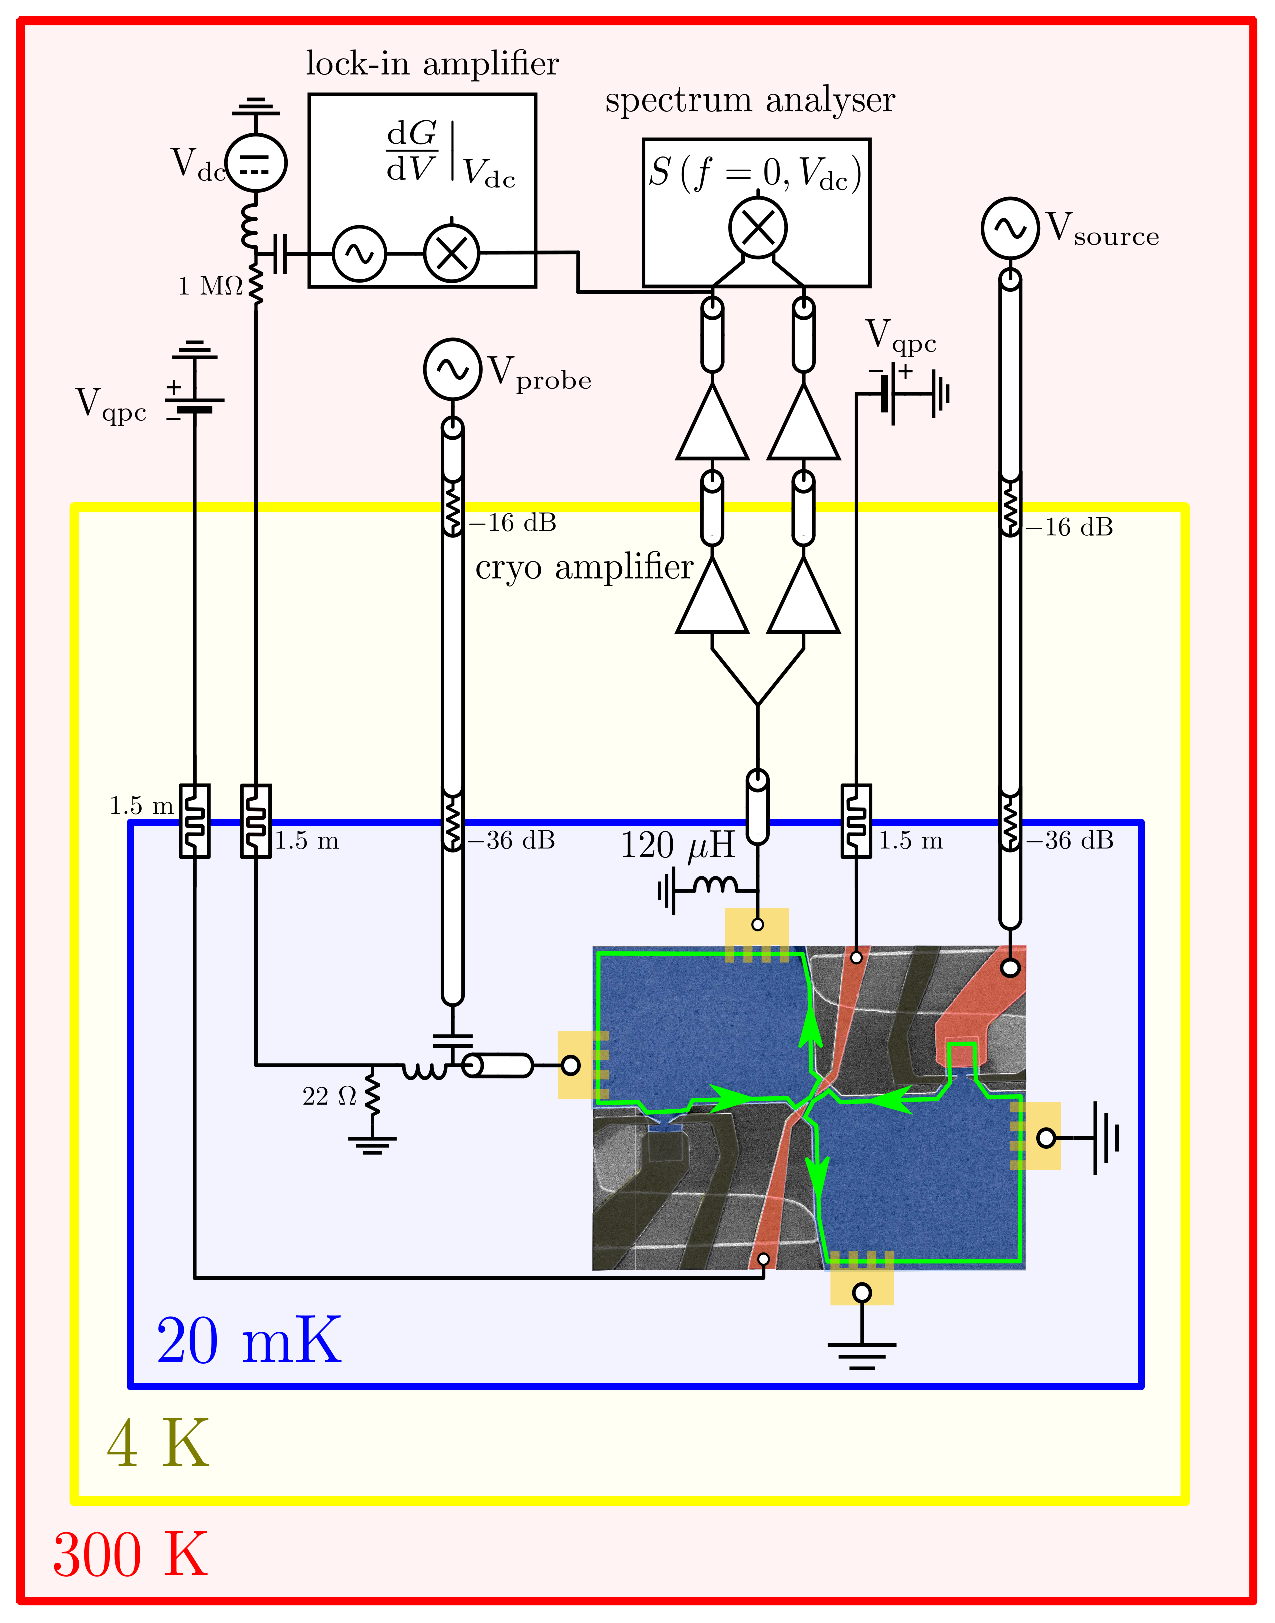
\includegraphics[width = 10cm]{./chap1/set-up_bruit_BF_pour_tomo.eps}
	\caption{\textbf{Experimental set-up used to performed electronic wavefunction tomography.} This schematic is separated in four regions: the red part at 300 K which is the exterior of the dilution fridge; the yellow part at 4K and the blue part at 20 mK which are inner stage of the dilution fridge; the sample SEM picture in false color which is the object studied. On the sample the 2D electron gas is coloured in blue, the gates in red, the Ohmic contacts are added in yellow, the outer edge-channel in green. Injection lines for RF signals V$_{\mathrm{source}}$, V$_{\mathrm{probe}}$, and DC signals V$_{\mathrm{dc}}$, V$_{\mathrm{qpc}}$ are represented with their attributed attenuation and thermalisation. The measurement lines and the two measurement instruments: a spectrum analyser to get the low frequency noise, a lock-in amplifier to check the quantum point contact transmission, are detailed.}
	\label{fig: le set-up}
\end{figure}

The first step is to generate electronic wavefunctions in a 1D conductor.
The 1D conductor used for this purpose is the outer edge channel of the integer quantum Hall effect.
This outer edge channel is drawn in green on the false colour picture of the sample in figure Fig. \ref{fig: le set-up}.
It is formed by applying a $2.6$ T magnetic field perpendicular to the 2D electron gas represented in dark blue in the sample picture.
At this magnetic field, the filling factor of the 2D electron gas is $3$.
It implies that there are also two inner edge channels not represented on the sample picture.
%All these edge channels are ballistic 1D conductor, because they have no longitudinal resistance.
All these edge channels are ballistic 1D conductor, as shown by their vanishing longitudinal resistance.
They are also chiral, so they guide the electronic excitations in the wanted direction.
%But because of electron-electron interactions between edge channels for example\cite{ferraro2014real,freulon2015hong,marguerite2016decoherence}, the waveform of signal propagating are deformed.
However electron-electron interactions between edge channels \cite{ferraro2014real,freulon2015hong,marguerite2016decoherence} deform the waveform of propagating signal.
We explain below how we control this deformation of the signal in order to generate specific wavefunctions in the edge channel at a specific location.
As the aim is to visualize wavefunctions, we need to send a state with only few of them, and not a statistical mixed state between a large number of them.
%These states are non-classical states, and they correspond to excitations which are faster than the thermal blurring.
These states are non-classical states, and they require that emission time is smaller than the thermal time $\frac{h}{k_{\mathrm{B}}T_{\mathrm{elec}}} \sim 1$ ns.
The instrument used to apply voltage waveform is an arbitrary wave generator (AWG).
The analogue bandwidth of the one used is of 25 GHz, this corresponds to an energy scale of around 100 $\upmu$eV.
To lower thermal blurring, the sample is cooled by a dilution fridge.
The first stages of the fridge allow the system to reach a temperature of 4 K thanks to a pulse tube cooler.
Experimental parts at this temperature are on a yellow background in the figure Fig. \ref{fig: le set-up}.
The last stages reach a temperature of around 20 mK with a dilution unit.
On a blue background are displayed the elements at this temperature and in particular the sample.
The electrons in the 2D electron gas are at a higher temperature of $T_{\mathrm{elec}} \sim 50$ mK than the sample.
Even with this higher electronic temperature than the dilution fridge temperature the thermal excitations are at an energy scale of 4 $\upmu$eV, well below the analogue bandwith of the arbitrary wave generator.

\subsubsection*{Input lines}

The experimental set-up uses two inputs with one source controlled by the voltage $V_{\mathrm{source}}$ to generate wavefunctions, and one probe of reference voltages $V_{\mathrm{probe}}$ to image the wavefunctions.
To carry the voltage waveform from the instrument to the edge channel we use different input lines, see the figure Fig. \ref{fig: le set-up}.
The RF lines are used to bring the high frequency signals, they are connected to the output channels $V_{\mathrm{source}}$ and $V_{\mathrm{probe}}$ of the AWG.
They are attenuated by 16 dB before the 4 K stage and by 36 dB before the coldest stage, in order to attenuate the room temperature thermal noise coming from the instrument.
The zero frequency voltage $V_{\mathrm{dc}}$ is added thanks to a Bilt voltage source.
It is connected with a Bias Tee on a RF line through a DC line also filtered, thermalized, and attenuated by a voltage divider.
The separation of zero frequency and high frequency input lines allow using the DC line to apply bigger voltage than the maximum enabled by the RF line attenuation, as it is required in the previous chapter.
The detailed elements on each stage of these input lines are on the schematics of annexe figures \ref{fig: Input RF lines} and \ref{fig: Input DC lines}.
One edge channel is connected to input lines of $V_{\mathrm{probe}}$ and $V_{\mathrm{dc}}$ thanks to an Ohmic contact.
The opposite edge channel does not need a zero frequency component, so the voltage $V_{\mathrm{source}}$ is applied via a gate coloured in red \cite{misiorny2018shaping}.
This gate is capacitively coupled to the outer edge channel, it is the top gate of the mesoscopic capacitor \cite{gabelli2006violation}.
As already mentioned above for interactions between edge channels, the voltage pulses are also deformed by dispersive cables, connectors, bonding wires.
This deformation implies that the pulse shapes send at room temperature from the instrument output are very different than the one in the center of the sample.
A calibration links the two shapes and is used to compensate for all the voltage pulse deformations.
The source voltage is decomposed in 5 harmonics as in equation \eqref{eq: Fourier components of Vsource}.

\begin{equation}
V_{\mathrm{source}}\left(t\right) = \sum_{n=1}^{5} V_{n}\cos\left(2\pi n\nu t+\phi_{n}\right) \label{eq: Fourier components of Vsource}
\end{equation}

In the first result section \ref{sec: Results for single charge periodic Lorentzian pulses}, the pulse wanted is a periodic train of Lorentzian shape pulses \eqref{eq: voltage lorentzian train}.

\begin{equation}
V_{\mathrm{source}}\left(t\right) = \sum_{m = -\infty}^{+\infty} \frac{\frac{e}{\pi\tau}}{1+\left(\frac{t-mT}{\tau}\right)^{2}} \label{eq: voltage lorentzian train}
\end{equation}

It has the parameters of a repetition frequency of $\frac{1}{T} = \nu = 4$ GHz and a half width at half maximum of $\tau = 40$ ps. 
To generate this pulse with five harmonics the calibrations of amplitudes $V_{n}$ and phases $\phi_{n}$ are performed for each Fourier components separately.
The propagation along a channel of one Fourier component changes only the values of $V_{n}$ and $\phi_{n}$ \cite{bocquillon2013separation} that are calibrated thanks to noise measurements.
Before the amplitude and phase calibrations, the next two paragraphs detail the noise measurements.
%Because if we send a single sine excitation, than only its amplitude and phase are affected but it stays a sine excitation \cite{bocquillon2013separation}.
%So for each Fourier component we need to calibrate both its amplitude and its phase.



\subsubsection*{Noise measurement line}

In the centre of the sample, a quantum point contact (QPC) is used to access informations on excitations in the edge-channel.
It is formed by the two red gates in the centre of the sample in figure Fig.\ref{fig: le set-up}.
These two gates repeal the 2D electron gas below them, and bring together the two edges of the sample.
It forms at the central point between the gates a tunnel barrier for electrons in the edge channel.
Its transmission and reflection are adjusted thanks to the voltage $V_{\mathrm{qpc}}$ applied to the gates.
The lock-in amplifier, connected as in figure Fig. \ref{fig: le set-up}, can monitor the reflection value by measuring the backscattered signal at the quantum point contact, see figure Fig. \ref{fig: RF charac at 2} panel (b).
In this experiment the gate voltage $V_{\mathrm{qpc}}$ is chosen such that the quantum point contact is half transmitting.
This quantum point contact acts as a 50/50 beam splitter for electrons, with two incoming opposite edge channels excited with $V_{\mathrm{probe}}$ and $V_{\mathrm{source}}$, and two outgoing opposite edge channels.
The excitations are guided by the chiral edge channels toward the quantum point contact.
It randomly partitions them in the two output edge channels, so the electrons are randomly transmitted or reflected.
The measured quantity to access information on the excitations is the generated current shot noise in one output edge channel.
The measurement is performed around 1 MHz, which is equivalent to zero frequency because it is very small compared to thermal excitations $\frac{k_{B}T}{h} \sim 1$ GHz.
An Ohmic contact collects the current in the output edge channel.
It is connected to two high input impedance and low noise cryogenic amplifiers \cite{dong2014ultra} at 4 K stage.
In parallel with the input of the amplifiers, a coreless coil shifts the measurement frequency at 1.1 MHz, because it makes a resonant circuit with cables and amplifiers input capacitances.
The signal is then amplified again by room temperature low noise amplifiers.
A vector spectrum analyser computes the cross-correlations by multiplying the two signals together.
These cross correlations suppress the voltage noise of the amplifiers.
The value recorded is the noise power integrated in a band of 200 kHz centred at 1.1 MHz.

\subsubsection*{Gain calibration}

\begin{figure}[hptb]
	\begin{center}
		\begin{tabular}{c c c c}
			(a) & & (b) &  \\ 
			
			& 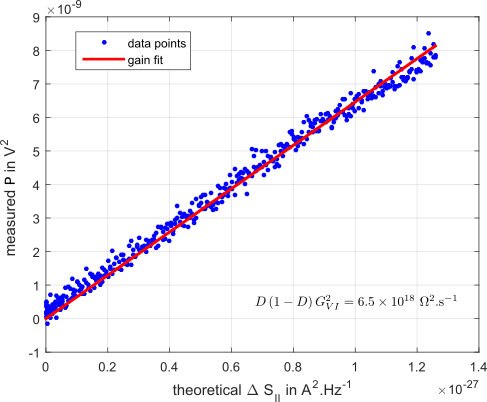
\includegraphics[width = 6cm]{./chap1/gain_noise_measurement} &
			& 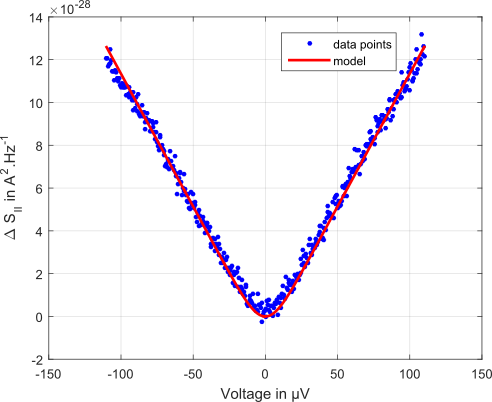
\includegraphics[width = 6cm]{./chap1/DC_shoit_noise_renormalized}
		\end{tabular} 
	\end{center}
	\caption{\textbf{Gain calibration of the low frequency noise measurement line.} \textbf{(a)} Comparison between measured and theoretically expected shot noise to obtain the gain. The noise power integrated on the acquisition band measured by the spectrum analyser in V$^{2}$ is plotted in blue points as a function of the calculated expected shot noise in A$^{2}$.Hz$^{-1}$ thanks to the knowledge of the DC voltage applied and equation \eqref{eq: DC excess shot noise}. The linear fit in red line gives the gain of the measurement line. \textbf{(b)} In blue points is plotted the shot noise data points measured and divided by the gain found in the panel (a) as a function of the applied DC voltage. They verify the equation \eqref{eq: DC excess shot noise} for DC shot noise with an electronic temperature $T_{\mathrm{elec}} = 50$ mK.}
	\label{fig: DC shot noise}
\end{figure}

%The gain of this noise measurement line is known by applying DC voltages.
The gain of this noise measurement line is calibrated by measuring the zero frequency current noise generated by a DC voltage.
When we apply only a DC voltage $V_{\mathrm{dc}}$, we can compute theoretically the zero frequency excess shot noise \eqref{eq: DC excess shot noise} at the quantum point contact output \cite{blanter2000shot}.

\begin{equation}
\Delta S_{II}\left(V_{\mathrm{dc}}\right) = 4\frac{e^{2}}{h}k_{\mathrm{B}}T_{\mathrm{elec}}D(1-D)\left(\frac{eV_{\mathrm{dc}}}{2k_{\mathrm{B}}T_{\mathrm{elec}}}\coth\left(\frac{eV_{\mathrm{dc}}}{2k_{\mathrm{B}}T_{\mathrm{elec}}}\right)-1\right) \label{eq: DC excess shot noise}
\end{equation}

In the measurement and in the calculation, we get the excess shot noise by subtracting the thermal noise when there is no excitation, here $\Delta S_{II}\left(V_{\mathrm{dc}}\right) = S\left(V_{\mathrm{dc}}\right)-S\left(V_{\mathrm{dc}}=0\right)$.
The excess shot noise is more directly linked to the excitations since the thermal noise is subtracted.
In figure Fig. \ref{fig: DC shot noise} (a), the measured excess noise power $P$ is plotted as a function of the calculated excess shot noise.
The linear red curve $P = \left(D\left(1-D\right)G^{2}_{VI}\right) \Delta S_{II}$ fits the blue data points, and its slope gives the noise measurement gain $D\left(1-D\right)G^{2}_{VI} = 6.5\times 10^{18}$ $\Omega^{2}$.s$^{-1}$ including the Fano factor $D(1-D)$ with transmission $D$.
On the panel (b), the shot noise divided by the Fano factor is plotted as a function of the DC voltage applied $V_{\mathrm{dc}}$.
The blue data points are renormalized by the measured gain and they are consistent with the calculated shot noise at an electronic temperature $T_{\mathrm{elec}} = 50$ mK in red.

\subsubsection*{Amplitude calibration}

\begin{figure}[hptb]
	\begin{center}
		\begin{tabular}{c c c c}
			(a) & & (b) &  \\ 
			
			& 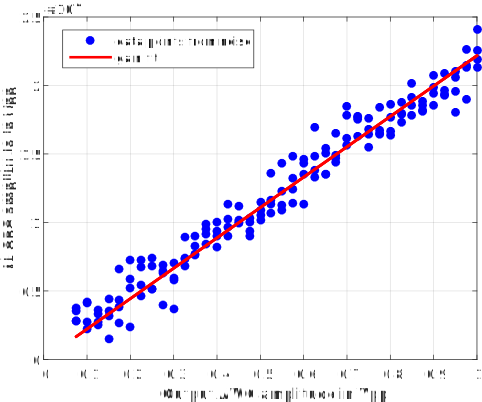
\includegraphics[width = 6cm]{./chap1/gain_injection_4GHz} &
			& 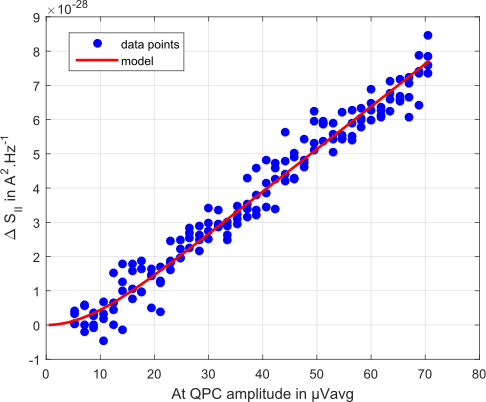
\includegraphics[width = 6cm]{./chap1/PA_shoit_noise_renormalized_4GHz}
		\end{tabular} 
	\end{center}
	\caption{\textbf{Attenuation calibration of the RF input line of voltage V$_{\mathrm{source}}$ at the frequency of 4 GHz.} \textbf{(a)} In blue points is represented the voltage amplitude at the quantum point contact deduced from shot noise measurement as a function of the voltage amplitude of the instrument output. The instrument is an arbitrary wave generator emitting a sine voltage at 4 GHz. The red line is a linear fit whose slope is the line attenuation. \textbf{(b)} Blue data points are the measured photo-assisted shot noise as a function of the output voltage of the instrument multiplied by the line attenuation. Red line is the approximate model of the photo-assisted shot noise by the DC shot noise of the averaged rectified voltage. This graphs shows that at this frequency and voltage range, the approximation is valid compared to the measurement precision.}
	\label{fig: PA shot noise}
\end{figure}

%To calibrate one harmonic amplitude, the DC voltage is replaced by a sinus voltage at the chosen frequency.
To calibrate one source and probe amplitude $V_{n}$ of the equation \eqref{eq: Fourier components of Vsource}, the DC voltage is replaced by a sinus voltage at the chosen frequency.
When varying the amplitude of the sine at the instrument output, we measure the photo-assisted shot noise $\Delta S_{II}$ generated by the excitation thanks to the noise gain calibration \cite{bize2003bruit}.
We also calculate the amplitude of a sinus $V_{n}$ giving the same photo-assisted shot noise, and the ratio between the amplitude of the instrument output and the calculated voltage giving the same noise is the attenuation.
In the figure Fig. \ref{fig: PA shot noise}, there is an example of a sinus at 4 GHz.
At this frequency, with an electronic temperature of 50 mK, the range of amplitude of 50 $\upmu$V, and the precision of the measurement, we can approximate the photo-assisted noise by the DC excess shot noise \eqref{eq: DC excess shot noise} of the averaged voltage $V_{\mathrm{avg}}$ applied on half a period.
This average voltage is proportional to the amplitude with $V_{\mathrm{avg}} = \frac{2n}{T}\int_{0}^{T/(2n)}V_{n}\sin\left(2\pi n\nu t\right)\mathrm{d}t = \frac{2}{\pi}V_{n}$.
In the panel (a), the average voltage deduced from excess shot noise measurement is plotted as a function of the amplitude of the 4 GHz sine voltage at the output of the instrument.
The average voltage is deduced from the noise measurement by inverting the equation \eqref{eq: DC excess shot noise}, with the additional approximation that $\coth\left(\frac{eV_{\mathrm{avg}}}{2k_{\mathrm{B}}T_{\mathrm{elec}}}\right) \sim 1$, which gives the equation \eqref{eq: voltage avg from noise}.

\begin{equation}
V_{\mathrm{avg}} = \frac{h}{2e^{3}}\left(\Delta S_{II}+4\frac{e^{2}}{h}k_{\mathrm{B}}T_{\mathrm{elec}}\right) \label{eq: voltage avg from noise}
\end{equation}

The slope of the fitted linear red curve gives the attenuation of the 4 GHz harmonic between the instrument and the central quantum point contact.
The panel (b) validates the different approximations with the blue data points of the photo-assisted shot noise which are consistent with the red line of the calculated excess shot noise thanks to the formula \eqref{eq: DC excess shot noise}.

\subsubsection*{Phase calibration}

\begin{figure}[hptb]
	\begin{center}
		\begin{tabular}{c}
			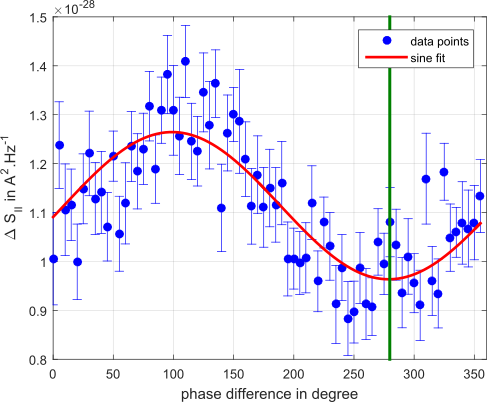
\includegraphics[width = 6cm]{./chap1/phase_calibration_8GHz}
		\end{tabular} 
	\end{center}
	\caption{\textbf{Phase difference calibration between 4 GHz and 8 GHz sine voltage.} The blue point values are the excess shot noise when an 8 GHz sinus voltage is added to the 4 GHz sinus voltage phase reference. They are plotted as a function of the phase of the 8 GHz sinus, and fitted by a sine function in red line. The fit parameters allow compensating the phase difference between the reference 4 GHz and the 8 GHz harmonics.}
	\label{fig: phase calibration}
\end{figure}

After calibrating the amplitudes $V_{n}$ of each harmonic, we calibrate the phase $\phi_{n}$ of each harmonic in equation \eqref{eq: Fourier components of Vsource}.
In our example the 4 GHz sinus is used as a phase reference so $\phi_{1} = 0$.
And all other harmonics have a relative phase $\phi_{n>1}$ compared to this excitation.
The second harmonic at 8 GHz is for example injected in addition to the reference first harmonic 4 GHz sinus.
When two excitations are sent on the quantum point contact, we realize an electronic Hong-Ou-Mandel experiment.
Like in optics, it has been shown for electrons in this system \cite{hong1987measurement,bocquillon2013} that the excess shot noise depends on the overlap of the two excitations.
At fixed amplitude for both harmonics, the overlap between the two sinus excitations at 4 GHz and 8 GHz is governed by their relative phase.
Depending on whether the sinus are injected in the same or opposite edge channels, they are in phase at a minimum or a maximum of excess shot noise.
When the ratio of frequencies of the harmonic is even, we need to apply a DC voltage in addition to get the variation of the excess noise.
%In figure Fig. \ref{fig: phase calibration} the excess noise of an added 8 GHz sinus switched ON and OFF to the reference 4 GHz sinus is plotted as a function of the 8 GHz sinus phase at the instrument output.
In figure Fig. \ref{fig: phase calibration} the excess noise of an added 8 GHz sinus to the reference 4 GHz sinus is plotted as a function of the 8 GHz sinus phase $\phi_{2}$ of the instrument output.
On the graph we remark a periodic modulation of the excess shot noise with the phase as expected.
And the phase corresponding to the minimum of noise, noted by a green dashed line, is the phase adjustment at which the harmonic arrives in phase with the reference at the quantum point contact.
With this method we are able to calibrate amplitude and phase of each sine at all frequencies sent in the inputs edge-channel.
Thanks to these calibrations, we can compensate attenuation and dephasing of each harmonic to get the chosen pulse \eqref{eq: voltage lorentzian train} at the quantum point contact location.
%In the first result section \ref{sec: Results for single charge periodic Lorentzian pulses}, the pulse sent is a periodic train of Lorentzian shape pulses.
%It is generated with a repetition frequency of 4 GHz and a half width at half maximum of 40ps, thanks to the calibration of harmonics.

\subsection{The measurement}

\subsubsection*{The Hong-Ou-Mandel interferometer}

\begin{figure}[hptb]
	\begin{center}
		\begin{tabular}{c c c c c}
			(a) & & & & \\
			& \includegraphics[width = 1.5cm]{./chap1/dessin_HOM_a_1}
			&  & &  \\
			(b) & & & & \\
			& 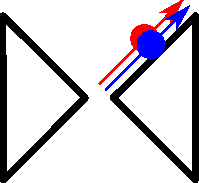
\includegraphics[width = 1.5cm]{./chap1/dessin_HOM_b_1}
			& \includegraphics[width = 1.5cm]{./chap1/dessin_HOM_b_2} 
			& \includegraphics[width = 1.5cm]{./chap1/dessin_HOM_b_3}
			& \includegraphics[width = 1.5cm]{./chap1/dessin_HOM_b_4} \\
			(c) & & & & \\
			& \includegraphics[width = 1.5cm]{./chap1/dessin_HOM_c_1}
			& \includegraphics[width = 1.5cm]{./chap1/dessin_HOM_c_2} 
			& \includegraphics[width = 1.5cm]{./chap1/dessin_HOM_c_2} 
			& \includegraphics[width = 1.5cm]{./chap1/dessin_HOM_c_3}
		\end{tabular} 
	\end{center}
	\caption{ \textbf{Schematics of principle of the Hong-Ou-Mandel electronic interferometer.} \textbf{(a)} Two electrons are injected in the opposite inputs of a quantum point contact. \textbf{(b)} If the two electrons are distinguishable, four outcomes are possibles and the number of electrons in an output edge channel fluctuates. It induces low frequency current noise. \textbf{(c)} If the two electrons are indistinguishable, then the outcomes where the electrons are in the same output edge-channel are forbidden due to fermionic statistic, and the low frequency current noise is suppressed.}
	\label{fig: HOM principle}
\end{figure}

In the above subsection, the Hong-Ou-Mandel effect has already been introduced in the phase calibration, to get information on the phase difference between two harmonics.
The sample geometry is the electronic analogue of the Hong-Ou-Mandel interferometer and has already been used to show an interference effect between electrons from separate sources \cite{bocquillon2013}.
These interference effects allowed probing electronic interactions during the propagation along quantum Hall effect edge channels \cite{freulon2015hong}.
In these experiments the noise is also measured and it has been demonstrated that the excess shot noise suppression is proportional to the overlap between input electronic states of the Hong-Ou-Mandel interferometer.
The principle of this effect is illustrated in the figure Fig. \ref{fig: HOM principle}.
If one sends two electrons as sketched on the panel (a), they are four outcomes possible see panel (b): two where they take the same exit, and two where they take different exits.
But if the electrons are indistinguishable, due to the Fermi statistics they never take the same exit as shown on the panel (c).
So in the situation of identical electrons there is always one electron in each exit.
The current does not fluctuate and the zero frequency shot noise is suppressed.
The overlap of electronic states involved in this effect has been quantified in reference \cite{marguerite2017two} by the equation \eqref{eq: excess shot noise and overlap} which links the excess shot noise and the Wigner distribution of the two electronic states.

\begin{equation}
\Delta S_{II} = -4\frac{e^{2}}{h}\nu\int_{-\infty}^{+\infty}\mathrm{d}E\int_{0}^{T}\mathrm{d}t \Delta W_{\mathrm{S}}\left(E,t\right)\Delta W_{\mathrm{P}}\left(E,t\right) \label{eq: excess shot noise and overlap}
\end{equation}

%In this equation the excess shot noise \eqref{eq: def excess noise for tomography} is the total noise where both the source $(S)$ and the probe $(P)$ are switched on minus the noise with only one turned on.
In this equation the excess noise $\Delta S_{II}$ is equal to the difference between several noise, as in \eqref{eq: def excess noise for tomography}, in order to get only the interference term between source and probe \cite{marguerite2017two}.
The first difference is the noise $S_{II}\left(S:\mathrm{on},P:\mathrm{on}\right)$ when both source and probe are generated minus the noise $S_{II}\left(S:\mathrm{off},P:\mathrm{on}\right)$ when only the probe is generated and the source is replaced by a zero voltage excitation $V_{\mathrm{source}} = 0$.
This difference suppress the contribution of the probe alone.
The second difference subtracts to the result of the first difference, the noise $S_{II}\left(S:\mathrm{on},P:\mathrm{off}\right)$ of the source alone with a probe replaced by a zero voltage excitation $V_{\mathrm{probe}} = 0$ minus the noise $S_{II}\left(S:\mathrm{off},P:\mathrm{off}\right)$ when both source and probe are zero voltage sources $V_{\mathrm{source}} = V_{\mathrm{probe}} = 0$.
This second difference subtracts the contribution of the source alone.

\begin{equation}
\Delta S_{II} = S_{II}\left(S:\mathrm{on},P:\mathrm{on}\right)-S_{II}\left(S:\mathrm{off},P:\mathrm{on}\right)-\left(S_{II}\left(S:\mathrm{on},P:\mathrm{off}\right)-S_{II}\left(S:\mathrm{off},P:\mathrm{off}\right)\right) \label{eq: def excess noise for tomography}
\end{equation}

All these noises are divided by the Fano factor $D\left(1-D\right)$ since it is included in the noise measurement line gain by its calibration.

The excess Wigner distribution $\Delta W\left(E,t\right)$ is the Wigner distribution minus the Wigner distribution of the Fermi sea $f_{T_{\mathrm{elec}}}\left(E\right)$ at the electronic temperature $T_{\mathrm{elec}}=50$ mK, see \eqref{eq: excess Wigner at finite temp}.

\begin{equation}
\Delta W\left(E,t\right) = W\left(E,t\right) - f_{T_{\mathrm{elec}}}\left(E\right) = W\left(E,t\right) - \frac{1}{1+e^{-E/k_{\mathrm{B}}T_{\mathrm{elec}}}} \label{eq: excess Wigner at finite temp}
\end{equation}

As explained in the previous section \ref{sec: Wigner distribution and electronic wavefunctions}, the Fermi sea is the reference state which is present even if we do not excite the system.
So the shot noise measurements give information on the excess Wigner distribution added to this reference state at finite temperature.

\subsubsection*{The tomography protocol}

\begin{figure}[hpbt]
	\centering
	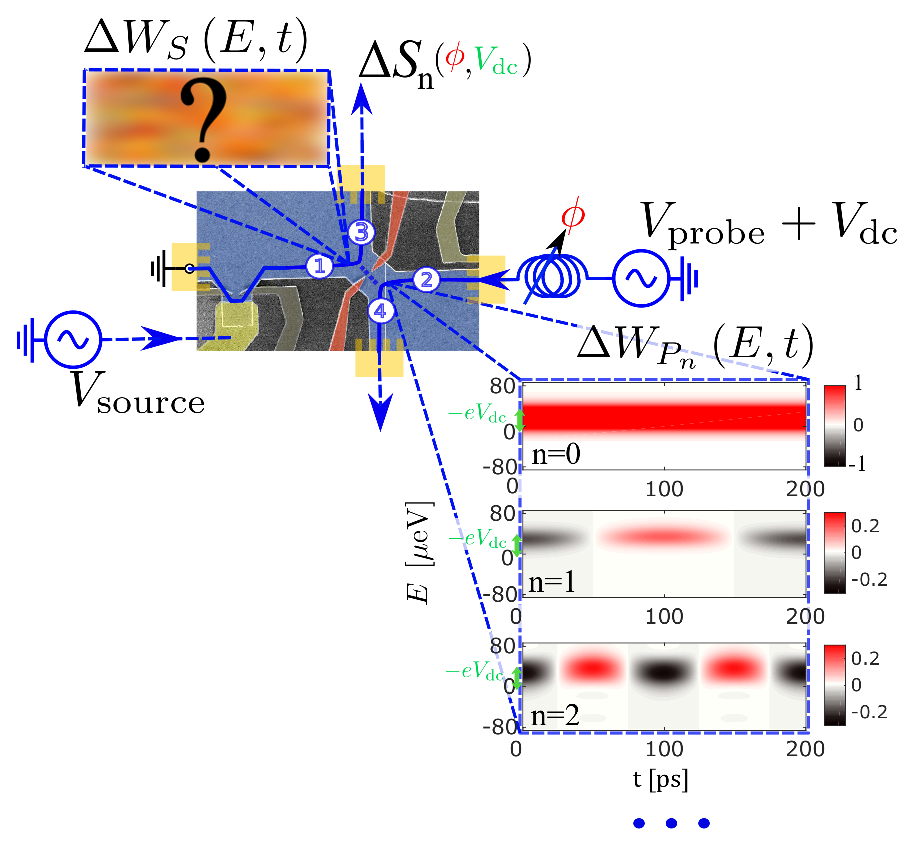
\includegraphics[width = 13cm]{./chap1/figure_principe_tomo.eps}
	\caption{\textbf{Tomography protocol implementation schematics.} In the bottom left, there is a voltage source applied on a yellow top gate. This gate excite the edge-channel 1, in order to get the unknown source Wigner distribution $\Delta W_{S}$ at the central quantum point contact location. This quantum point contact is formed by top gates coloured in red. The edge channel 1 meet at this point the other input edge channel 2. With an Ohmic contact the known $n$ probes Wigner distribution $\Delta W_{P_{n}}$ of phase $\phi$ and energy offset $-eV_{\mathrm{dc}}$ are sent in edge channel 2. And the measured noise in output edge channel 3 for all parameters $n$,$\phi$,$V_{\mathrm{dc}}$ are overlaps between known $\Delta W_{P_{n}}$ and searched $\Delta W_{S}$.}
	\label{fig: principe de la tomographie}
\end{figure}

\begin{figure}[hptb]
	\begin{center}
		\begin{tabular}{c c c c}
			(a) & & (b) &  \\ 
			
			& 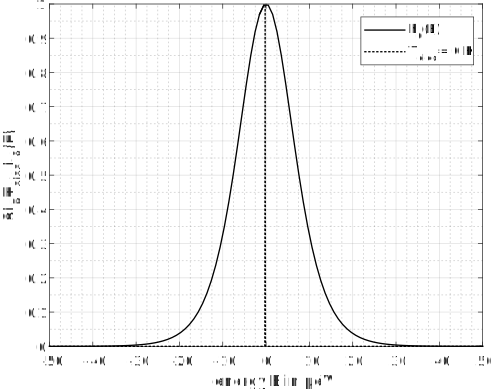
\includegraphics[width = 6cm]{./chap1/convolution_h_0} &
			& 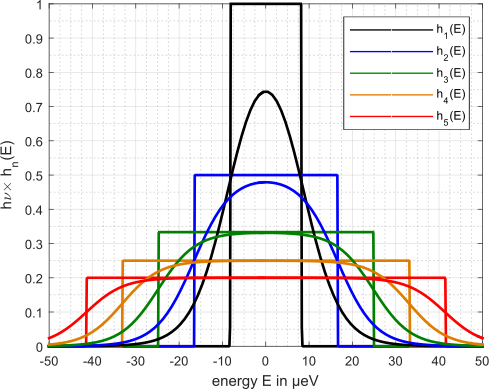
\includegraphics[width = 6cm]{./chap1/convolution_h_1_to_5}
		\end{tabular} 
	\end{center}
	\caption{\textbf{Convolution functions at a temperature of $T_{\mathrm{elec}} = 50$ mK and a fundamental frequency of $ \nu = 4$ GHz.} \textbf{(a)} The function $h_{0}\left(E\right)$ defined in equation \eqref{eq: convolution spectro} is plotted. The function is multiplied by $2k_{\mathrm{B}}T_{\mathrm{elec}}$ to get a function plotted between 0 and 1. The black line corresponds to a temperature of 50 mK and it is compared to a temperature of 0 K in dashed line. \textbf{(b)} The functions $h_{n}\left(E\right)$ defined in equation \eqref{eq: excess wigner probe n h function} are plotted for n from 1 in black to 5 in red. The functions are multiplied by $h\nu$ to be bounded between 0 and 1. The dashed lines are the zero temperature functions.}
	\label{fig: convolution function}
\end{figure}

Following the protocol of \cite{grenier2011single} a succession of overlap measurements between the unknown source excess Wigner distribution $\Delta W_{S}$ and known probe Wigner distribution $\Delta W_{P}$, allows measuring the searched excess Wigner distribution $\Delta W_{S}$.
This is a tomography protocol where the 2D function $\Delta W_{S}$ is reconstructed from a collection of overlaps with different probes.
The chosen probes are DC voltages and sine voltages.
As seen in the above subsection, they are the easiest to calibrate and to generate because they consist of only one harmonic.
Each probe is at one multiple of the source fundamental frequency $\nu$ so they enable reconstructing the excess Wigner distribution $\Delta W_{S}$ harmonic per harmonic.
The Wigner distribution is expanded as a Fourier transform along the time variable by equation \eqref{eq: time Fourier transform of Wigner}.

\begin{equation}
\Delta W_{S}\left(E,t\right) = \Delta W_{S,0}\left(E\right)+2\sum_{n=1}^{5}\Re\left(\Delta W_{S,n}\left(E\right)\exp\left(2\pi i n \nu t\right)\right) \label{eq: time Fourier transform of Wigner}
\end{equation}

The first probe is a DC voltage, its Wigner distribution is the same as the Fermi sea but shifted by a chemical potential of $\mu = -eV_{\mathrm{dc}}$.
So the excess Wigner distribution of the probe is the difference between two Fermi functions \eqref{eq: Wigner dc probe} and is plotted on the panel $n = 0$ of panels of $\Delta W_{P_{n}}$ in the figure Fig. \ref{fig: principe de la tomographie}.
\begin{equation}
\Delta W_{P_{0}}\left(E,t\right) = f_{T_{\mathrm{elec}}}\left(E-\mu\right)-f_{T_{\mathrm{elec}}}\left(E\right) = \frac{1}{1+e^{-\left(E-\mu\right)/k_{\mathrm{B}}T_{\mathrm{elec}}}}-\frac{1}{1+e^{-E/k_{\mathrm{B}}T_{\mathrm{elec}}}} \label{eq: Wigner dc probe}
\end{equation}
It does not depend on time $\Delta W_{P_{0}}\left(E,t\right) = \Delta W_{P_{0}}\left(E\right)$ so the excess noise measured $\Delta S_{0}\left(V_{\mathrm{dc}}\right)$ probes the average on time of the source Wigner distribution $\Delta W_{S,0}\left(E\right)$ \eqref{eq: noise spectro}.

\begin{equation}
\Delta S_{0}\left(V_{\mathrm{dc}}\right) = -4\frac{e^{2}}{h}\int_{-\infty}^{+\infty}\mathrm{d}E\Delta W_{S,0}\left(E\right)\Delta W_{P_{0}}\left(E\right)\;\mathrm{with}\;\Delta W_{S,0}\left(E\right) = \nu\int_{0}^{T}\mathrm{d}t \Delta W_{\mathrm{S}}\left(E,t\right) \label{eq: noise spectro}
\end{equation}

The derivative of the excess noise versus $V_{\mathrm{dc}}$ is equal to a convolution product \eqref{eq: convolution spectro} between $\Delta W_{S,0}\left(E\right)$ and a function $h_{0}\left(E\right)$ of width $2k_{\mathrm{B}}T_{\mathrm{elec}}$.
The function $h_{0}\left(E\right)$ is plotted in figure Fig \ref{fig: convolution function} panel (a) for the electronic temperature $T_{\mathrm{elec}} = 50$ mK corresponding to the measurements and it tends towards a Dirac function at  $T_{\mathrm{elec}} = 0$ K.

\begin{equation}
\frac{\mathrm{d}\Delta S_{0}}{\mathrm{d}V_{\mathrm{dc}}} =  2\frac{e^{3}}{h}\int_{-\infty}^{+\infty} \mathrm{d}E \Delta W_{S,0}\left(E\right)h_{0}\left(E+eV_{\mathrm{dc}}\right)\;\mathrm{with}\;h_{0}\left(E\right) = \frac{1}{k_{\mathrm{B}}T_{\mathrm{elec}}\left(1+\cosh\left(\frac{E}{k_{\mathrm{B}}T_{\mathrm{elec}}}\right)\right)} \label{eq: convolution spectro}
\end{equation}

From the above equation, we measure the average over time of the Wigner distribution $\Delta W_{S,0}\left(E\right)$, which is also the marginal equal to the occupation.

The other probes give information on time dependent part of the Wigner distribution.
For other probes we apply a sinus modulation in addition to the dc voltage $V_{n}\left(t\right) = V_{\mathrm{dc}}+V_{\mathrm{ac}}\cos\left(2\pi n \nu t + \phi\right)$ with $n$ from 1 to 5.
Its excess Wigner distribution for small amplitude $V_{\mathrm{ac}}$ is at first order \eqref{eq: excess wigner probe n}.
Two examples for which $n = 1$ and $2$ are represented in the figure Fig. \ref{fig: principe de la tomographie} in panels of $\Delta W_{P_{n}}\left(E,t\right)$.

\begin{equation}
\Delta W_{P_{n}}\left(E,t\right) = \Delta W_{P_{0}}\left(E,t\right)-eV_{\mathrm{ac}}\cos\left(2\pi n \nu t + \phi\right)h_{n}\left(E+eV_{\mathrm{dc}}\right) \label{eq: excess wigner probe n}
\end{equation}

\begin{equation}
\mathrm{with}\;h_{n}\left(E\right)=\frac{1}{nh\nu}\left(\frac{1}{1+e^{-\left(E-\frac{nh\nu}{2}\right)/k_{\mathrm{B}}T_{\mathrm{elec}}}}-\frac{1}{1+e^{-\left(E+\frac{nh\nu}{2}\right)/k_{\mathrm{B}}T_{\mathrm{elec}}}}\right) \label{eq: excess wigner probe n h function}
\end{equation}

When we subtract the excess noise measurement of two opposite probe phases $\phi$ of $0$ and $\pi$ or $\frac{\pi}{2}$ and $\frac{3\pi}{2}$, we get the convolution products \eqref{eq: convolution real part tomo} \eqref{eq: convolution imag part tomo} between the $n$ time harmonic of the Wigner distribution $\Delta W_{S,n}\left(E\right)$ \eqref{eq: convolution real part tomo Re def} \eqref{eq: convolution imag part tomo Im def} and the function $h_{n}\left(E\right)$ \eqref{eq: excess wigner probe n h function} of width $nh\nu$.
The functions $h_{n}\left(E\right)$ for the 5 harmonics $n$ from 1 to 5 are plotted in figure Fig. \ref{fig: convolution function} panel (b).
On the graph we remark that they are gate functions at 0 K and with a temperature of 50 mK their edges are rounded.

\begin{equation}
\Delta S_{n,\phi=0}\left(V_{\mathrm{dc}}\right)-\Delta S_{n,\phi=\pi}\left(V_{\mathrm{dc}}\right) = 8\frac{e^{3}V_{\mathrm{ac}}}{h}\int_{-\infty}^{+\infty}\mathrm{d}E\Re\left(\Delta W_{S,n}\left(E\right)\right)h_{n}\left(E+eV_{\mathrm{dc}}\right) \label{eq: convolution real part tomo}
\end{equation}

\begin{equation}
\mathrm{with}\;\Re\left(\Delta W_{S,n}\left(E\right)\right) = \nu\int_{0}^{T}\mathrm{d}t \Delta W_{S}\left(E,t\right)\cos\left(2\pi n \nu t\right) \label{eq: convolution real part tomo Re def}
\end{equation}

\begin{equation}
\Delta S_{n,\phi=\pi/2}\left(V_{\mathrm{dc}}\right)-\Delta S_{n,\phi=3\pi/2}\left(V_{\mathrm{dc}}\right) = 8\frac{e^{3}V_{\mathrm{ac}}}{h}\int_{-\infty}^{+\infty}\mathrm{d}E\Im\left(\Delta W_{S,n}\left(E\right)\right)h_{n}\left(E+eV_{\mathrm{dc}}\right) \label{eq: convolution imag part tomo}
\end{equation}

\begin{equation}
\mathrm{with}\;\Im\left(\Delta W_{S,n}\left(E\right)\right) = \nu\int_{0}^{T}\mathrm{d}t \Delta W_{S}\left(E,t\right)\sin\left(2\pi n \nu t\right) \label{eq: convolution imag part tomo Im def}
\end{equation}

The figure Fig. \ref{fig: principe de la tomographie} summarizes the tomography protocol discussed above.
In the edge channel 1, the gate injects an unknown Wigner distribution $\Delta W_{S}\left(E,t\right)$ at the quantum point contact.
In the edge channel 2, we inject thanks to an Ohmic contact different probes numbered by n.
The excess Wigner distribution $\Delta W_{P_{\mathrm{n}}}\left(E,t\right)$ of the first probes $n = 0, 1, 2$ are plotted in the figure Fig. \ref{fig: principe de la tomographie}.
%From the edge channel 3 the excess shot noise is a measurement of the overlaps between the searched Wigner distribution and the probes.
By measuring the excess shot noise $\Delta S_{\mathrm{n}}$ generated at the output channel 3, we extract the overlap between $\Delta W_{S}\left(E,t\right)$ and $\Delta W_{P_{\mathrm{n}}}\left(E,t\right)$, see \eqref{eq: excess shot noise and overlap}.


\subsubsection*{Noise measurement results}

\begin{figure}[hptb]
	\begin{center}
		\begin{tabular}{c c c c}
			(a) & & (b) &  \\ 
			
			& 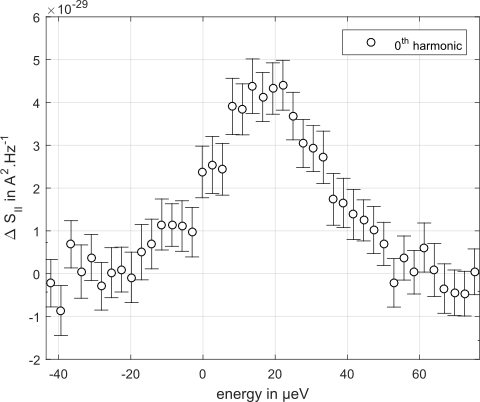
\includegraphics[width = 6cm]{./chap1/noise_spectro_leviton_1e_40ps} &
			& 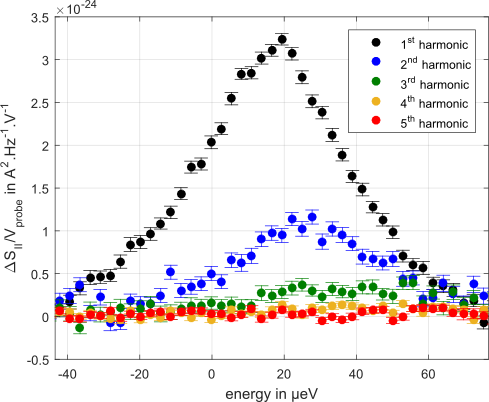
\includegraphics[width = 6cm]{./chap1/noise_tomo_leviton_1e_40ps}
		\end{tabular} 
	\end{center}
	\caption{\textbf{Shot noise measurement results for a periodic train of Lorentzian pulses carrying one elementary charge.} \textbf{(a)} Excess shot noise of the $0^{\mathrm{th}}$ harmonic divided by the Fano factor $D\left(1-D\right)$. The excess shot noise is the noise difference between the pulse source injected with a DC probe voltage minus the noise of the DC probe voltage alone. The energy axis is the applied DC probe voltage shifted by the missing DC component of the source $h\nu$.  \textbf{(b)} Excess shot noise of all other harmonics divided by the corresponding probe voltage amplitude. The excess shot noise is the noise difference between the noise of sources and probes injected in phase and in opposite phase. The energy axis is the same as in (a).}
	\label{fig: measured noise}
\end{figure}

The excess shot noise results are plotted in figure Fig. \ref{fig: measured noise}.
The data points are the one used for the results discussed in the section \ref{sec: Results for single charge periodic Lorentzian pulses}.
In the panel (a) there is the noise when the source and the DC voltage $V_{\mathrm{dc}}$ are applied minus the noise when only the DC voltage is applied, as a function of the energy $-eV_{\mathrm{dc}}+h\nu$.
The energy is shifted by $h\nu$ because the excitation is done by a gate so the DC part of the pulse is included in the analysis by shifting the applied DC voltage of the probes by $\frac{h\nu}{e}$.
In the panel (b), the points correspond to the excess shot noise difference between the probes phase $\phi$ equals 0 and $\pi$ divided by the probe amplitude $V_{\mathrm{ac}}$.
In the equation \eqref{eq: convolution real part tomo}, these points measure the real part of the time harmonics of the Wigner distribution.
For the results presented in this chapter, the imaginary parts are equal to zero, due to the shape of the pulses.
In the annexe \ref{sec: An asymetric pulse with exponentially decreasing current}, the case of an asymmetric exponential pulse is presented where imaginary parts are different from zero.

\subsection{The deconvolution}

From the time harmonics $\Delta W_{S,n}$, the Wigner distribution is expressed by a time Fourier transform \eqref{eq: time Fourier transform of Wigner} but the shot noise measurements in the figure Fig. \ref{fig: measured noise} are not a direct measurement of $\Delta W_{S,n}$.
The equations \eqref{eq: convolution spectro} and \eqref{eq: convolution real part tomo} show that the measurements are the convolution products between the time harmonics $\Delta W_{S,n}\left(E\right)$ and functions $h_{n}\left(E\right)$.
A deconvolution method is needed to invert the convolution product equations.
This standard inversion problem is also present in other situations such as image deblurring, 3D reconstruction \cite{chapdelaine20173d}.
We benefit from these developments to adapt and apply them to our specific case with the help of the C. Chapdelaine and A. Mohammad-Djafari from Laboratoire des signaux et systèmes at Centrale-Supélec.
The method chosen is in a Bayesian framework \cite{mohammad2015bayesian} and it is explained in detail here.
The convolution is modelled as a matrix product \eqref{eq: matrix product for convolution} with the discretization given by the measurement points plus a random measurement noise $N$ which follows a Gaussian distribution of variances $V_{e}$ given by the estimation of measurement error bars.

\begin{equation}
\Delta S = H\Delta W + N \label{eq: matrix product for convolution}
\end{equation}

With the above equation, we also express a probability distribution $p\left(\Delta S \left|\right. \Delta W, V_{e} \right)$ for the measurements $\Delta S$ which follows a Gaussian probability distribution called the likelihood \eqref{eq: likelihood}.

\begin{equation}
p\left(\Delta S \left|\right. \Delta W, V_{e}  \right) \propto \exp\left(-\frac{1}{2}\left||\Delta S - H\Delta W\right||^{2}_{V_{e}}\right)\;\mathrm{with}\;\left||X\right||^{2}_{V} = \sum_{i}^{}\frac{x^{2}_{i}}{v_{i}} \label{eq: likelihood}
\end{equation}

As the searched quantity is $\Delta W$, the probability distribution of interest, called posterior distribution, is the one of $\Delta W$ knowing the measurements $\Delta S$.
The Bayes' theorem \eqref{eq: Bayes'theorem} links the two probability distributions.

\begin{equation}
p\left(\Delta W \left|\right. \Delta S, V_{e} \right) p\left(\Delta S\right) = p\left(\Delta S \left|\right. \Delta W, V_{e}  \right) p\left( \Delta W \right) \label{eq: Bayes'theorem}
\end{equation}

It also introduces two other probability distributions.
The model evidence $p\left(\Delta S\right)$ does not depend on the solution $\Delta W$, so it will be ignored in the following.
The prior $p\left( \Delta W \right)$ allows adding a priori information to get a solution.
%The chosen prior information is the excess Wigner distribution is smaller at high energies than at energies close to the Fermi level.
We choose the following prior information: the excess Wigner distribution is smaller at high energies than at energies close to the Fermi level.
This prior information is expressed as a Gaussian prior distribution \eqref{eq: prior distribution} with energy dependent variances $V_{f}$.

\begin{equation}
p\left( \Delta W \left|\right. V_{f} \right) \propto \exp\left(-\frac{1}{2}\left||\Delta W\right||^{2}_{V_{f}}\right) \label{eq: prior distribution}
\end{equation}

These variances are initialized by a Gaussian function \eqref{eq: initialization hyper-prior} of amplitude $v_{f}$ and width $w$ for its energy dependence.

\begin{equation}
V_{f}\left(E\right) = v_{f}\exp\left(-\left(\frac{E}{w}\right)^{2}\right) \label{eq: initialization hyper-prior}
\end{equation}

Thanks to the precedent equations \eqref{eq: likelihood}, \eqref{eq: Bayes'theorem}, \eqref{eq: prior distribution}, \eqref{eq: initialization hyper-prior}, the posterior distribution is expressed by equation \eqref{eq: posterior MAP}.

\begin{equation}
p\left(\Delta W \left|\right. \Delta S, V_{e}, V_{f} \right) \propto p\left(\Delta S \left|\right. \Delta W, V_{e}\right)p\left(\Delta W \left|\right. V_{f} \right) \propto \exp\left(-\frac{1}{2}\left||\Delta S-H\Delta W\right||^{2}_{V_{e}}-\frac{1}{2}\left||\Delta W\right||^{2}_{V_{f}}\right) \label{eq: posterior MAP}
\end{equation}

The solution defined as the most likely $\Delta W$ knowing measurement values $\Delta S$, their variances $V_{e}$, and the a priori information $V_{f}$, is the argument which maximizes the above posterior distribution \eqref{eq: posterior MAP}.
In this case the solution is given analytically by equation \eqref{eq: MAP solution}.

\begin{equation}
\Delta W = \left(H^{\top}V_{e}^{-1}H+V_{f}^{-1}\right)^{-1}H^{\top}V_{e}^{-1}\Delta S \label{eq: MAP solution}
\end{equation}

In practice the variances $V_{f}\left(E\right)$ are not known, so the usual hypothesis is made that a probability distribution is assigned to variances, \cite{mohammad2015bayesian}.
The variances are assumed to follow inverse-gamma probability distributions \eqref{eq: inverse-gamma distribution} of fixed scale parameters $\beta\left(E\right)$ and the shape parameter $\alpha$.

\begin{equation}
p\left( V_{f}\left(E\right) \left|\right. \beta\left(E\right),\alpha \right) \propto V_{f}\left(E\right)^{-\alpha-1}\exp\left(-\frac{\beta\left(E\right)}{V_{f}\left(E\right)}\right) \label{eq: inverse-gamma distribution}
\end{equation}

$\alpha$ is chosen to adjust the dependence of $V_{f}\left(E\right)$ with the initialization \eqref{eq: initialization hyper-prior}.
The closer it is to -1, the less the variances depend on initialization.
$\beta\left(E\right)$ are fixed in order to have the maximum of the inverse-gamma equals the initial value of $V_{f}\left(E\right)$.

Other informations are the Pauli exclusion principle and the Cauchy-Schwartz inequalities, which come from the definition of the Wigner distribution \cite{ferraro2013wigner}.
%The Pauli exclusion principle enforce the occupation to take values between 0 and 1.
%The Cauchy-Schwartz inequalities avoid that coherences between different energy states leads to a probability of occupation of one state below 0 or above 1.
These two properties of the Wigner distribution bound the results accessible for the different time harmonics.
The Pauli exclusion principle implies that the occupation marginal is bounded between 0 and 1 \eqref{eq: Pauli exclusion principle}.
And the occupation marginal is equal to the Fermi distribution plus the 0$^{\mathrm{th}}$harmonic of the excess Wigner distribution.

\begin{equation}
0 \leq f_{T_{\mathrm{elec}}}\left(E\right)+\Delta W_{0}\left(E\right) \leq 1 \label{eq: Pauli exclusion principle}
\end{equation}

The Cauchy-Schwartz inequalities \eqref{eq: electron Cauchy-Schwartz inequality} \eqref{eq: hole Cauchy-Schwartz inequality} express the idea that there are no coherences between two states if there are not occupied.

\begin{equation}
\left|\Delta W_{n}\left(E\right)\right|^{2} \leq \left(f_{T_{\mathrm{elec}}}\left(E+\frac{nh\nu}{2}\right)+\Delta W_{0}\left(E+\frac{nh\nu}{2}\right)\right)\left(f_{T_{\mathrm{elec}}}\left(E-\frac{nh\nu}{2}\right)+\Delta W_{0}\left(E-\frac{nh\nu}{2}\right)\right) \label{eq: electron Cauchy-Schwartz inequality}
\end{equation}

\begin{equation}
\left|\Delta W_{n}\left(E\right)\right|^{2} \leq \left(1-f_{T_{\mathrm{elec}}}\left(E+\frac{nh\nu}{2}\right)-\Delta W_{0}\left(E+\frac{nh\nu}{2}\right)\right)\left(1-f_{T_{\mathrm{elec}}}\left(E-\frac{nh\nu}{2}\right)-\Delta W_{0}\left(E-\frac{nh\nu}{2}\right)\right) \label{eq: hole Cauchy-Schwartz inequality}
\end{equation}

In inequality \eqref{eq: electron Cauchy-Schwartz inequality}, the right term is the product of the occupation of states at energies $E+\frac{nh\nu}{2}$ and $E-\frac{nh\nu}{2}$.
The left term is the $n^{\mathrm{th}}$ coefficient of the time Fourier transform of the Wigner distribution.
So it is also equal to the $\epsilon = nh\nu$ value of the energy coherence function $\Delta_{0}G\left(E+\frac{\epsilon}{2},E-\frac{\epsilon}{2}\right)$ defined in the equation \eqref{eq: definition Glauber function}.
And it is the coherence between the two energy states $E+\frac{nh\nu}{2}$ and $E-\frac{nh\nu}{2}$.
In inequality \eqref{eq: hole Cauchy-Schwartz inequality}, the right term is the product of the occupation of hole states at energies $E+\frac{nh\nu}{2}$ and $E-\frac{nh\nu}{2}$, because it is one minus the electron occupation.
And the left term is still the coherence between these two states.
To take into account these two inequalities, the solution has to be found in the domain defined by them.
Inside this domain the solution is then chosen as the most likely couple of $\Delta W$ and $V_{f}$ knowing the measurement points $\Delta S$, their error bars with $V_{e}$ and parameters $\beta$ and $\alpha$.
This gives the probability distribution \eqref{eq: full posterior distribution}.

\begin{equation}
p\left(\Delta W, V_{f}\left|\right.\Delta S, V_{e}, \beta, \alpha\right) \propto p\left(\Delta S\left|\right.\Delta W, V_{e}\right)p\left(\Delta W \left|\right. V_{f}\right)p\left(V_{f}\left|\right.\beta,\alpha\right) \label{eq: full posterior distribution}
\end{equation}

The most likely couple of $\Delta W$ and $V_{f}$, called joint maximum a posteriori \cite{ayasso2010joint,zhao2016joint}, is searched by an algorithm detailed in Algorithm \ref{alg : Detailed algorithm}.

The two variables $\Delta W$ and $V_{f}$ are not handled simultaneously but this algorithm performs an alternate maximization of first $p\left(\Delta W\left|\right.V_{f}, \Delta S, V_{e}, \beta, \alpha\right)$ and then $p\left(V_{f}\left|\right.\Delta W, \Delta S, V_{e}, \beta, \alpha\right)$.

The first maximization as a function of $\Delta W$ is performed thanks to a projected gradient step \cite{bertsekas1997nonlinear,figueiredo2007gradient}.
It consists of calculating the gradient of minus the logarithm of the first distribution $-\ln\left(p\left(\Delta W\left|\right.V_{f}, \Delta S, V_{e}, \beta, \alpha\right)\right)$, project it to stay in the box constraint imposed by \eqref{eq: electron Cauchy-Schwartz inequality} \eqref{eq: hole Cauchy-Schwartz inequality}, compute the optimum displacement, and perform one descent step.

The maximization of the second distribution $p\left(V_{f}\left|\right.\Delta W, \Delta S, V_{e}, \beta, \alpha\right)$ is obtained with the derivatives of the distribution with respect to each coefficient $V_f(E)$ when $\Delta W$ is fixed.
These derivatives are equal to zero for $V_{f}\left(E\right) = \frac{1}{\alpha+3/2}\left(\beta\left(E\right)+\frac{1}{2}\Delta W\left(E\right)^{2}\right)$, so the maximization is the update of $V_f(E)$ with the above formula.
%The formula $V_{f}\left(E\right) = \frac{1}{\alpha+3/2}\left(\beta\left(E\right)+\frac{1}{2}\Delta W\left(E\right)^{2}\right)$ gives the value of $V_{f}$ which puts equal to zero the derivative, so its maximization is its update with the above formula.
%This algorithm performs an alternate maximization of first $p\left(\Delta W\left|\right.V_{f}, \Delta S, V_{e}, \beta, \alpha\right)$ and then $p\left(V_{f}\left|\right.\Delta W, \Delta S, V_{e}, \beta, \alpha\right)$.
%The first maximization is performed thanks to a projected gradient step \cite{bertsekas1997nonlinear,figueiredo2007gradient}.
%It consists of calculating the gradient of minus the logarithm of the first distribution $-\ln\left(p\left(\Delta W\left|\right.V_{f}, \Delta S, V_{e}, \beta, \alpha\right)\right)$, project it to stay in the box constraint imposed by \eqref{eq: electron Cauchy-Schwartz inequality} \eqref{eq: hole Cauchy-Schwartz inequality}, compute the optimum displacement, and perform one descent step.
%The maximization of the second distribution $p\left(V_{f}\left|\right.\Delta W, \Delta S, V_{e}, \beta, \alpha\right)$ is an update of $V_{f}$ values with the formula $V_{f}\left(E\right) = \frac{1}{\alpha+3/2}\left(\beta\left(E\right)+\frac{1}{2}\Delta W\left(E\right)^{2}\right)$.
A more detailed explanation of the motivations of deconvolution algorithms and their developments is done in annexe \ref{sec: Bayesian approach for deconvolution in electronic tomography}.
In the figure Fig. \ref{fig: after deconvolution}, the deconvolution results of the measurements in yhe figure Fig. \ref{fig: measured noise} are plotted.
We remark that the deconvolved points are less spread in energy than the raw measurements but some oscillations appear due to the noise amplification by the deconvolution process.
The presented Algorithm \ref{alg : Detailed algorithm} aims at correcting the blurring in energy by the convolution process without amplifying too much measurement noise.

\begin{figure}[hpbt]
	\centering
	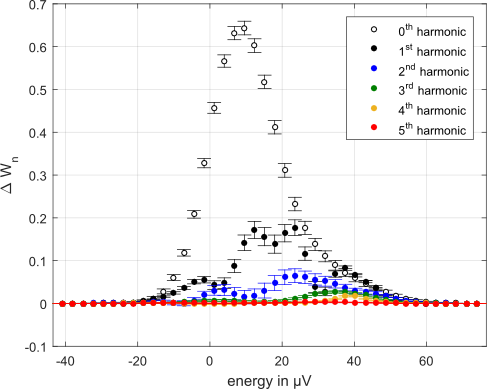
\includegraphics[width = 6.5cm]{./chap1/wigner_harmonic_deconvoluted}
	\caption{\textbf{Deconvolution results of the shot noise measurement of Lorentzian pulses.}  The deconvolution results are plotted with the same color as their input data in figure Fig.\ref{fig: measured noise}. The energy axis is the same as for noise measurement. For the $0^{\mathrm{th}}$ harmonic the excess Wigner distribution of the missing source DC voltage component $h\nu$ is added. The $0^{\mathrm{th}}$ harmonic also has the characteristic that the inverse problem includes a derivative calculation of the input data in addition to the deconvolution. The energy spread of the different harmonics are smaller than for measurements.}
	\label{fig: after deconvolution}
\end{figure}

%In the excess shot noise data we have the information on the excess Wigner distribution but via the equation $\Delta S_{II} = -e^{2}\nu \iint \frac{dEdt}{h} W_{S}(E,t)W_{P}(E,t)$.
%Which can also be written for each harmonic after integration other time and displaying the $V_{dc}$ dependence as $\Delta S_{n}(V_{dc}) = -\frac{e^{2}}{h} \int dE W_{n,S}(E)h_{n,P}(E-eV_{dc})$.
%The measurements $\Delta S_{n}(V_{dc}) $ are a convolution product between the known probe function $h_{n,P}$ and the unknown Wigner distribution harmonic $W_{n,S}(E)$.
%To solve this equation in presence of measurement noise, we used a Bayesian framework.
%Than we get the solution with respect to the finite temperature Fermi sea of the system without excitations.
%So we add this Fermi sea at finite temperature, with the same temperature as the one of the probes, deduce from shot noise measurement of a DC bias.

\newpage

\begin{algorithm}[H]
	\caption{Algorithm used to deconvolve shot noise measurements $\Delta S_{n}$ and obtain excess Winger function harmonics $\Delta W_{S,n}$.}
	\label{alg : Detailed algorithm}
	\begin{algorithmic}
		\STATE{Compute Pauli or Cauchy-Schwartz bounds $B_{n}\left(E\right)$}
		\STATE{Choose amplitude $v_{f}$ and width $w$ of prior \eqref{eq: initialization hyper-prior} for $V_{f}\left(E\right)$}
		\STATE{initialize $\beta$ with $\beta(E) = \left(\alpha+1\right)V_{f}\left(E\right)$}
		
		\STATE{Compute the minimum of criterion $-\ln\left(p\left(\mathbf{\Delta W}_{S,n}  \left|\right.\mathbf{V}_{f},
			\mathbf{\Delta S}_{n},\mathbf{V}_{e} \right) \right)$}
		\STATE{$\mathbf{\Delta W}_{S,n} =
			\left(\mathbf{H}^{\top}\mathbf{V}^{-1}_{e}\mathbf{H}+
			\mathbf{V}^{-1}_{f}\right)^{-1}\mathbf{H}^{\top}\mathbf{V}^{-1}_{e}\mathbf{\Delta
					S}_{n}$}
		\STATE{Project the solution inside the box given by bounds $B_{n}\left(E\right)$:}
		\STATE{$\Delta W_{S,n}\left(E\right) := \min\left(\Delta W_{S,n}\left(E\right),B_{n}\left(E\right)\right)$}
		\STATE{and $\Delta W_{S,n}(E) := \max(\Delta W_{S,n}(E),-B_{n}(E))$}
		\REPEAT
		\STATE{Compute the gradient of criterion $-\ln\left(p\left(\mathbf{\Delta W}_{S,n}  \left|\right.\mathbf{V}_{f},
			\mathbf{\Delta S}_{n},\mathbf{V}_{e} \right) \right)$}
		\STATE{
			
			$\nabla \left(\mathbf{ \Delta W}_{S,n}\right)
			= -\mathbf{H}^{\top}\mathbf{V}^{-1}_{e}\left(\mathbf{\Delta S}_{n}
			-\mathbf{H}\mathbf{\Delta W}_{S,n}\right)
			+\mathbf{V}^{-1}_{f}\mathbf{\Delta
				W}_{S,n}
			$
		}
		\STATE{Project the gradient $\mathrm{\textbf{P}}\nabla\left(\mathbf{ \Delta W}_{S,n}\right) $ to stay in the box-constraint}
		\IF{$|\Delta W_{S,n}(E)| \geq B_{n}(E)$ and $\Delta W_{S,n}(E)*\nabla\left( \Delta W_{S,n}\right) (E) \leq 0$}
		\STATE{$\mathrm{P}\nabla\left( \Delta W_{S,n}\right)(E) = 0$}
		\ELSE
		\STATE{$\mathrm{P}\nabla\left(\Delta W_{S,n}\right)(E) = \nabla\left(\Delta W_{S,n}\right)(E)$}
		\ENDIF
		\STATE{Compute the furthest displacement $d_{\infty}$
			in the box along $\mathrm{\textbf{P}}\nabla\left( \mathbf{\Delta W}_{S,n} \right)$ direction}
		\FORALL{$\mathrm{P}\nabla\left(\Delta W_{S,n}\right)(E) \neq 0$}
		\STATE{$d_{\infty} := \min\left(\frac{B_{n}(E)-\Delta W_{S,n}(E)}{\mathrm{P}\nabla\left(\Delta W_{S,n}\right)(E)},
			d_{\infty}\right)$
		}
		\ENDFOR
		\STATE{Compute the optimum displacement $d_{0}$ along $\mathrm{\textbf{P}}\nabla\left( \mathbf{\Delta W}_{S,n}\right) $ direction}
		\STATE{$
			d_{0} = \left\|\mathrm{\textbf{P}}\nabla\left(
			\mathbf{\Delta W}_{S,n}\right)\right\|^{-2}
			\left( \left\|\mathbf{H}\mathrm{\textbf{P}}\nabla\left(
			\mathbf{\Delta
				W}_{S,n}\right)\right\|^{2}_{\mathbf{V}_{e}}
			\right.
			+\left.\left\|\mathrm{\textbf{P}}\nabla\left( \mathbf{\Delta
				W}_{S,n}\right)\right\|^{2}_{\mathbf{V}_{f}}\right)$}
		
		\STATE{Compute one projected descent gradient step}
		\STATE{$\mathbf{\Delta W}_{S,n} := \mathbf{\Delta W}_{S,n}
			- \min(d_{0},d_{\infty})\mathrm{\textbf{P}}\nabla\left( \mathbf{\Delta W}_{S,n}\right) $}
		
		\STATE{update $\mathbf{V}_{f}$ to minimize $-\ln\left(p\left( \mathbf{V}_{f} \left|\right.\mathbf{\Delta W}_{S,n}, \mathbf{\beta}, \alpha  \right) \right)$ }
		\STATE{$V_{f}(E) := \frac{\beta(E)+\frac{1}{2}\Delta W_{S,n}(E)^{2}}{\alpha+\frac{3}{2}}$}
		
		
		\UNTIL $-\ln\left(p\left(\mathbf{\Delta W}_{S,n}, \mathbf{V}_{f} \left|
		\mathbf{\Delta S}_{n},\mathbf{V}_{e}, \mathbf{\beta}, \alpha \right. \right) \right) $
		is minimized
	\end{algorithmic}
\end{algorithm}

\newpage

\section{\texorpdfstring{Results for single charge periodic Lorentzian pulses}{Results for single charge periodic Lorentzian pulses} \label{sec: Results for single charge periodic Lorentzian pulses}}

As proposed by Levitov and co-authors \cite{levitov1996electro}, we can generate a single electron state at T = 0K by applying a specific Lorentzian shape voltage.
This induces a single electronic excitation on top of the Fermi sea.
Following the experimental method presented above, we engineer a train of Lorentzian pulse \eqref{eq: voltage lorentzian train} carrying a single charge 1e at the temperature of $T_{\mathrm{elec}} = 50$ mK, a frequency repetition of $\nu = 4$ GHz, and a half-width at half-maximum of $\tau = 40$ ps.
Then we measure its Wigner distribution by following the precedent procedure and the reconstructed distribution is plotted in figure Fig. \ref{fig: wigner du 1e 40ps} panel (a).

\subsection{Wigner distribution}

\begin{figure}[hpbt]
	\begin{center}
		\begin{tabular}{c c c c}
		(a) & & (b) &  \\ 
		& 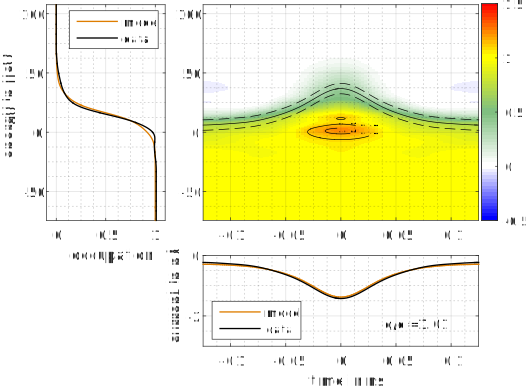
\includegraphics[width = 6.5cm]{./chap1/wigData_leviton_40ps_1e_51mK_Projected_Gradient_Method} &
		& 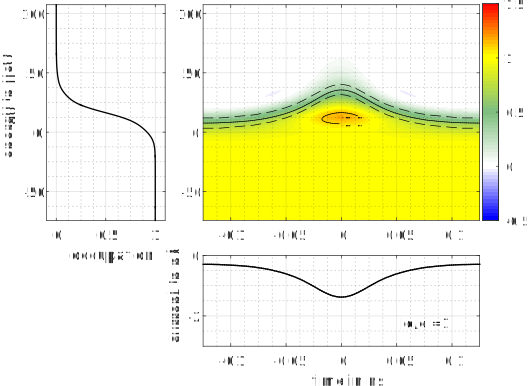
\includegraphics[width = 6.5cm]{./chap1/wigTheory_leviton_40ps_1e_50mK_6th_harm}
		\end{tabular} 
	\end{center}
	\caption{\textbf{Wigner distribution of a periodic train of Lorentzian pulses carrying one elementary charge.} \textbf{(a)} The horizontal time axis range is of one period of the 4 GHz repetition rate of pulses. The current, plotted in the bottom panel in black, is a Lorentzian pulse of 40 ps half width at half maximum. The integral of the current on one period is equal to one elementary charge. In the left panel, the occupation is plotted as a function of the vertical energy axis in black line, and is bounded between 0 and 1. The orange lines are current and occupation from the panel (b). The Wigner distribution is plotted in function of both time and energy. White and yellow colours indicate a value of 0 or 1. Green shows values between 0 and 1. Blue and red are below 0 and above 1 non-classical values. The black line is the time varying chemical potential deduced from the measured current $-eV(t) = -\frac{h}{e}I(t)$ and dashed lines are the same curve shifted by the thermal energy $\pm \frac{k_{\mathrm{B}}T_{\mathrm{elec}}}{e}$ \textbf{(b)} Calculations of the model Wigner distribution are plotted with the same axis and legends.}
	\label{fig: wigner du 1e 40ps}
\end{figure}

The first thing we check with the Wigner distribution is if we correctly send the expected current in the edge-channel.
For that we look at the current marginal of the Wigner distribution in the figure Fig. \ref{fig: wigner du 1e 40ps} panel (a).%, and we have a Lorentzian pulse of charge 1e per pulse.
We can check that we indeed generate a Lorentzian pulse carrying 1e charge per pulse.
Second we can look at the second marginal, the occupation, and we can remark that is almost equal to 1 up to the Fermi energy chosen as the reference energy.
It means that, as expected, only electrons and no holes are emitted.
%So there is only electrons emitted.
We can then look at the Wigner distribution, we can remark that the separation in the energy-time phase space between the presence of electrons and the absence of electrons, which is displayed in green by values between 0 and 1, follows approximately the time varying chemical potential $-eV(t) = \frac{h}{e}I(t)$ plotted in black line.
The typical width of this green region is of $5$ $\upmu$eV, which is consistent with the thermal excitation energy of $k_{B}T_{\mathrm{elec}}$ at 50mK.
The two dashed lines surrounding the green region are the black line $\pm \frac{k_{B}T_{\mathrm{elec}}}{e} = \pm5$ $\upmu$eV. 
Finally, one can notice that we are not just filling energy levels in yellow up to a time varying chemical potential $-eV(t)$ and let all above energy level empty.
The red spot at the pulse location corresponds to values above one, reaching $1.2$ as maximum value.
These values above one imply that we cannot interpret the Wigner distribution as a probability distribution, and so that a description of probability at simultaneously both conjugate variables energy and time is no more valid.
The state is not classical and requires a description in terms of wavefunctions.
%it is a non-classical state that requires a description in terms of wavefunctions.
This red zone appears when the typical time scale of the pulse $\tau = 40$ ps or the associated mean energy of the pulse is larger than thermal excitations $\frac{h}{\tau} \sim 20\times k_{B}T_{\mathrm{elec}}$.
This result is consistent with a non-interacting model plotted in the panel (b), where the voltage applied is modelled as a time dependent phase factor added to the Fermi sea \cite{grenier2011single}.
This is in agreement with the idea that we generate and measure the pulse at the same location, and so that we do not let time for interactions to occur during the propagation.



\subsection{Emission probabilities and inter-period coherences}

\begin{figure}[hptb]
	\begin{center}
		\begin{tabular}{c c c c}
			(a) & & (b) &  \\ 
			
			& 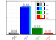
\includegraphics[width = 6.5cm]{./chap1/JnlData_leviton_40ps_1e_51mK_Projected_Gradient_Method_a} &
			& \includegraphics[width = 6.5cm]{./chap1/JnlData_leviton_40ps_1e_51mK_Projected_Gradient_Method_b}
		\end{tabular} 
	\end{center}
	\caption{\textbf{Weights of wavefunctions emission and coherences.} \textbf{(a)} Probabilities of emission of main wavefunctions. These values show there are only two electron wavefunction emitted (numbered 1 and 2), and no hole wavefunction. The light coloured bars with dashed edges are probabilities of the calculated Wigner distribution at the same temperature, and white bars with dot edges show that at zero temperature one pure state is emitted. \textbf{(b)} Inter-period coherences $g_{1}^{e}(l)$ and $g_{2}^{e}(l)$.%Coherence between the same electron wavefunctions only numbered 1 or only numbered 2 but they are shifted of $l$ periods.
	The coherence between periods decreases to zero after 5 periods. The same colour code of light points with dashed edges are calculated from model at the same temperature as measurements and white points with dotted edges correspond to zero temperature.}
	\label{fig: Jnl du 1e 40ps}
\end{figure}

To obtain the description in terms of wavefunctions we need to perform the diagonalization described in the above section.
This is done thanks to an algorithm written by Benjamin Roussel \cite{roussel2017autopsy}.
First it gives the probability of occupation of each wavefunctions.
The figure Fig. \ref{fig: Jnl du 1e 40ps} shows that the most populated hole has a probability of emission per period $0.03 \pm 0.01$ very close to zero.
This agrees with the idea that there are no holes excitations as we can see on the Wigner distribution.
Then we see that the electron wavefunctions populated are mainly the first two ones with $p_{1} = 0.83 \pm 0.01$ and $p_{2} = 0.18 \pm 0.01$, and the third most populated is $p_{3} = 0.02 \pm 0.01$ already very close to zero.
The fact there are these two wavefunctions populated between 0 and 1, and the sum of the two equals to one $p_{1}+p_{2} = 1.01 \pm 0.01$ indicates that we have a mixed state between these two wavefunctions.
The fact that we have a mixed state between only two wavefunctions and not a mixed state between large number of them agrees with the fact we have a non-classical Wigner distribution, because a mixed state of a large number of pure wavefunction is a classical state.
The fact there are two wavefunctions populated differs from the zero temperature case predicted by Levitov and co-authors \cite{levitov1996electro}, where only one pure wavefunction is expected.
This effect is not due to periodicity since in the works \cite{roussel2017autopsy} and \cite{moskalets2015first,moskalets2017single} it is demonstrated that at T=0K with a periodic train of Lorentzian pulses we still have a single pure wavefunction periodically emitted on top of the Fermi sea.
It is also not due to the finite number of harmonics, from 0 to 5, used to generate the Lorentzian pulse since with numerical calculations performed with the same number of harmonics we show that the probability of the most populated electron wavefunction tends towards $1$ when the temperature tends to $0$ K.
The emission of the extra wavefunction is thus caused by finite temperature effect, the numerical calculations at finite temperature give the same probabilities $p_{1} = 0.84$ and $p_{2} = 0.18$.
It should be noticed that the temperature effects are not associated with the emission of extra-electron hole pairs as studied in \cite{dubois2013minimal} but rather to the generation of a statistical mixture between two electronic wavefunctions.
%In this case the temperature does not generate extra electron-holes pairs as studied in \cite{dubois2013minimal}, but it generate a statistical mixed state of two wavefunctions.
Then we can look in the panel (b) of figure Fig. \ref{fig: Jnl du 1e 40ps} at the inter-period coherences of the two populated electronic wavefunctions.
We see that there are coherences only for a number of around five periods, this number corresponds to the ratio between the repetition rate of the Leviton train $h\nu$ over the thermal energy $k_{B}T_{\mathrm{elec}}$, here at $\nu = 4$ GHz and an electronic temperature of $50$ mK, we have $\frac{h\nu}{k_{B}T_{\mathrm{elec}}} = 4.8$.


\subsection{Wavefunctions}

\begin{figure}[hptb]
	\begin{center}
		\begin{tabular}{c c c c}
			(a) & & (b) &  \\ 
			
			& 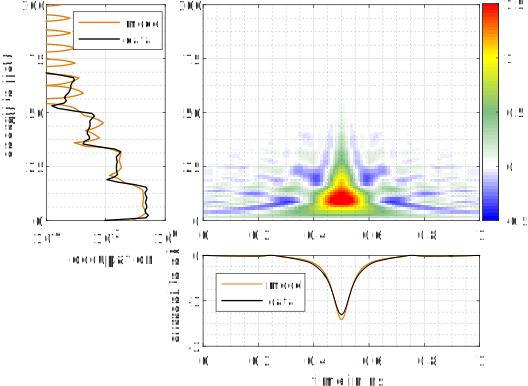
\includegraphics[width = 6.5cm]{./chap1/wannierwigData_leviton_40ps_1e_51mK_Projected_Gradient_Method-el-0} &
			& 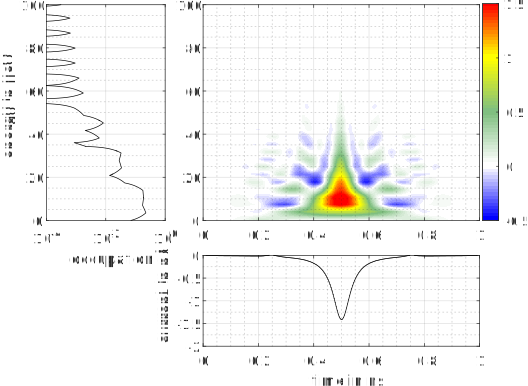
\includegraphics[width = 6.5cm]{./chap1/wannierwigTheory_leviton_40ps-el-0} \\
			(c) & & (d) &  \\
			& 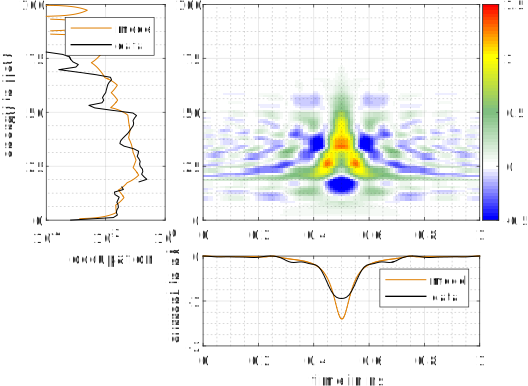
\includegraphics[width = 6.5cm]{./chap1/wannierwigData_leviton_40ps_1e_51mK_Projected_Gradient_Method-el-1} &
			& 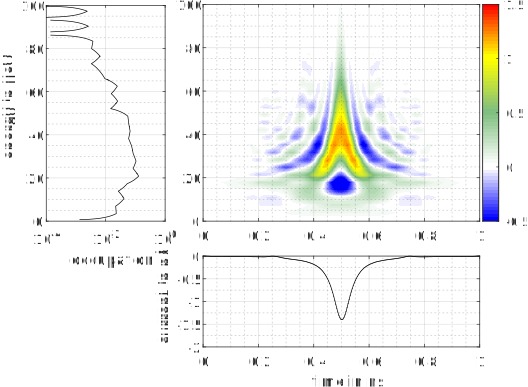
\includegraphics[width = 6.5cm]{./chap1/wannierwigTheory_leviton_40ps-el-1} \\
			
		\end{tabular} 
	\end{center}
	\caption{\textbf{Wigner distribution of wavefunctions involved in a periodic train of Lorentzian pulses carrying one elementary charge}. \textbf{(a)} Most populated electronic wavefunction numbered 1. It is a pure electronic state, only above Fermi level energies ($E>0$) are plotted. It has an overlap with theoretical 4 GHz periodic Lorentzian 40 ps width pulse at T = 0 K in the panel (b) of 0.98 . \textbf{(b)} Numercial calculations of a Lorentzian current pure state of width $\tau = 40$ ps. \textbf{(c)} Second emitted electronic wavefunction numbered 2. It is higher energy electronic states very close to the higher energy state in the basis of periodic Lorentzian pulse at T = 0 K with an overlap between these two of 0.94 . \textbf{(d)} The higher energy state in the basis of periodic pulse at T = 0 K. 
	This graph is plotted thanks to numerical calculations, first a Lorentzian current pulse carrying a charge 2e per pulse at T = 0 K is generated, then the diagonalization extracts two wavefunctions, and the higher energy wavefunction is selected. 
	%This graph is plotted thanks to numerical calculations where the wavefunctions are extracted from numerically generated data of a Lorentzian current pulse carrying a charge 2e per pulse. 
	%Numerical calculations of the higher energy Lorentzian pure state than panel (b).
	}
	\label{fig: wannier el du 1e 40ps}
\end{figure}

The algorithm of B. Roussel \cite{roussel2017autopsy} used to diagonalize the coherence function does not only give probabilities and coherences via the eigenvalues, but it also gives the corresponding wavefunctions via the eigenvectors. 
These wavefunctions are represented thanks to their Wigner distributions. They are plotted in the figure Fig.\ref{fig: wannier el du 1e 40ps} (a) and (b).
The energy scale of the plot is defined only for positive energy because as it is electronic wavefunction, their value is equal to zero for energy below the Fermi level.
%The time scale range is of 1ns so four times the period, because these wavefunctions are not periodic unlike the Wigner distribution plotted in Fig.\ref{fig: wigner du 1e 40ps} (a).
%But there are one of them at each periods.
The values taken by the Wigner distribution of the wavefunctions are displayed between -0.5 and 1.5.
As they correspond to Wigner distributions of pure states, the values below 0 in blue and above 1 in red are not blurred by a mixed state.

The occupation is plotted in log-lin scale for both wavefunctions.
First we see that the occupation is a step like function, the width in energy of these steps is of $16$ $\upmu$eV which is equal to $h\nu$ with here $\nu = 4$ GHz. These steps are due to the periodicity of the emission.
Because the voltage drive is periodic with a frequency $\nu$, we can only excite the systems per the amount of energy of $h\nu$.
This corresponds to the fact that the microwave photons generated in the RF cable and coupled to the edge channels have an energy which is a multiple of $h\nu$, and so the excitations generated by one or multiple photons are also quantized by the energy $h\nu$.
If we focus on the most populated wavefunction in the figure Fig.\ref{fig: wannier el du 1e 40ps} (a), the height of each energy steps of the energy marginal is also regular in the log-lin scale.
This indicates an exponential dependence on the steps value with the energy.
This reminds the results of the single Lorentzian pulse carrying a single charge at $T = 0$ K where an exponential shape is expected for the occupation, see the figure Fig. \ref{fig: Wigner Leviton}.
For the periodic case it has also been analytically computed at $T = 0$ K, the occupation is the same as for the Leviton but with a step like argument for the energy dependence, see figure Fig. \ref{fig: wannier el du 1e 40ps} panel (b).

The current, the time marginal, related to the probability of presence at a fixed time, is plotted in the figure Fig.\ref{fig: wannier el du 1e 40ps}.
The current is always negative, because it is a pure electronic wavefunction, so there are no holes leading to positive current.
The current pulses are spread to approximately one period of 0.25 ns, but they have different shapes.
The shape of the current of the most populated wavefunction in (a) is a Lorentzian shape, it gives another indicator of correspondence between this wavefunction and the analytical case of Lorentzian pulse.
The current in analytical calculation is the same for the single Lorentzian pulse and the periodic train of Lorentzian pulse, so there is no signature of the periodicity here compared to the occupation.
For the wavefunction (c), the current is a pulse of approximately the same width as for (a) and it looks like a Lorentzian pulse, but with some discrepancies.
%The integral of the current divided by $e$, is equal to the integral of the occupation, the number of electron, because they are both equals to the integral of the all Wigner distribution of the wavefunction, which is equal to one, as it is a single particle pure state.

What gives us the complete informations on these wavefunction is the Wigner distribution.
We can compute an overlap between the measured Wigner distribution of the most populated wavefunction (a) and the analytical calculation of wavefunction in a periodic train of Lorentzian pulses.
This overlap is $0.98$, it is very close to one.
So when we are driving a 1D conductor at $T_{\mathrm{elec}}=50$ mK with a train of Lorentzian pulse carrying one electric charge, we send $p_{0} = 0.83$ times the wavefunction corresponding to the zero temperature periodic case, with some coherent superposition between different periods up to approximately $\frac{hf}{k_{B}T_{\mathrm{elec}}} = 5$ periods.
For the second wavefunction emitted, we introduce the numerical case of a periodic train Lorentzian pulse carrying a charge of 2e at $T_{\mathrm{elec}} = 0$ K.
With this numerical result we compute two wavefunctions emitted per pulse, the first one is the same as the zero temperature one.
It corresponds to the measured wavefunction (a).
And the second wavefunction orthogonal to the last one is evaluated numerically.
Even if the current of the measured wavefunction (c) has small deviations with a Lorentzian, the two Wigner distributions are very similar and the overlap of the two is equal to $0.94$.
So the wavefunction emitted by an train of Lorentzian pulse excitation at $T_{\mathrm{elec}}=50$ mK is a mixed state between the zero temperature periodic Leviton wavefunction emitted with a probability of $p_{1} = 0.83 \pm 0.01$ and the higher energy periodic Leviton wavefunction emitted with a probability of $p_{2} = 0.18 \pm 0.01$.

\section{\texorpdfstring{Effects of Lorentzian pulses parameters}{Effects of Lorentzian pulses parameters} \label{sec: Effects of Lorentzian pulses parameters}}

In the above section, we have discussed the wavefunctions generated by a train of Lorentzian pulses.
%We can know change the parameters of this excitation and see how it affects the results.
In this section we investigate how we can engineer different wavefunctions by varying the parameters of the Lorentzian pulses.

\subsection{Twice shorter Lorentzian pulses}

The first parameter we can change is the width of the pulses, while keeping the same charge per pulse.
In our case we divide the width of the pulse by two, to get a Lorentzian pulse of half width at half maximum of $\tau = 25$ ps.
We also multiply the pulse amplitude by a factor 2 in order to keep the charge per pulse constant.
Technically, this implies to change the weight of the harmonics in the generated signal, what can be easily done with an Arbitrary Wave Generator (AWG) but in the limit of the amplitude range of the instrument. 
To get the following results, we repeat the same procedure of noise measurements and deconvolution.

\subsubsection*{Wigner distribution}

\begin{figure}[hpbt]
	\begin{center}
		\begin{tabular}{c c c c}
		(a) & & (b) &   \\ 
		& 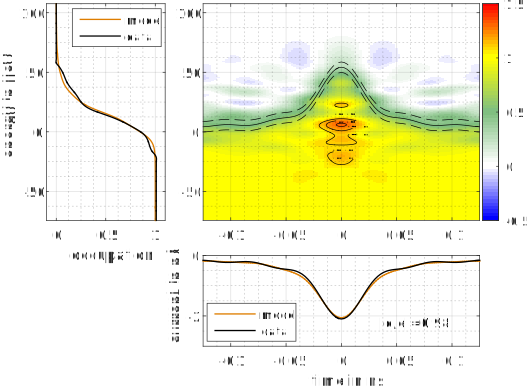
\includegraphics[width = 6.5cm]{./chap1/wigData_leviton_20ps_1e_51mK_Projected_Gradient_Method} &
		& 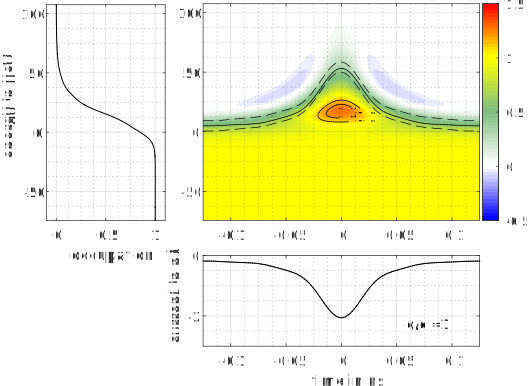
\includegraphics[width = 6.5cm]{./chap1/wigTheory_leviton_25ps_1e_50mK_6th_harm}
		\end{tabular} 
	\end{center}
	\caption{\textbf{Wigner distribution of a periodic train of shorter Lorentzian pulses carrying one elementary charge.} \textbf{(a)} Measured Wigner distribution for Lorentzian pulses of 25 ps half width at half maximum. The pulse width is twice shorter than in the previous section so it reaches twice higher energy and displays higher Wigner distribution maximum values of 1.3 compared to 1.2 previously. \textbf{(b)} Numerical calculations of the Wigner distribution with a Lorentzian pulse of width $\tau = 25$ ps}
	\label{fig: wigner du 1e 20ps}
\end{figure}

The Wigner distribution obtained is plotted in figure Fig.\ref{fig: wigner du 1e 20ps}.
If we first look at the current, we can remark as wanted that the width of the pulse is twice shorter and the height is twice larger.
The charge measurement by integrating the current indicates that it still carries a single charge per pulse $\left|\frac{q}{e}\right| = 0.98$.
The occupation function goes higher in energy because the voltage applied to the edge-state is higher at the maximum of the pulse.
As we are emitting a few number of states, we observe the limitation of the Heisenberg uncertainty relation \cite{heisenberg1949physical} with a twice shorter current pulse in time the spreading of the occupation in energy is twice bigger.
The occupation also shows some values below one at negative energies.
So there are some holes emitted.
On the Wigner distribution, we see that the pulse takes a shorter time window to occur and between two pulses there is space for the thermal excitations creating holes as displayed by green region at negative energies for the time $t = \pm \frac{T}{2}$ on the plot.
%In the Wigner distribution we also remark that the red zone in the middle of the pulse reach higher values around $1.3$ above one than for the case of a pulse twice larger, that was $1.2$.

\subsubsection*{Emission probabilities and inter-period coherences}

\begin{figure}[hptb]
	\begin{center}
		\begin{tabular}{c c c c}
			(a) & & &   \\ 
			 & 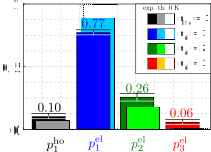
\includegraphics[width = 5cm]{./chap1/JnlData_leviton_20ps_1e_51mK_Projected_Gradient_Method_proba} &
			 &  \\
			 (b) & & (c) & \\
			 & \includegraphics[width = 5cm]{./chap1/JnlData_leviton_20ps_1e_51mK_Projected_Gradient_Method_coh_period} &
			 & \includegraphics[width = 5cm]{./chap1/JnlData_leviton_20ps_1e_51mK_Projected_Gradient_Method_coh_el_ho_0}
		\end{tabular} 
	\end{center}
	\caption{ \textbf{Weights of emission and coherences with a 20 ps width Lorentzian pulse.} \textbf{(a)} The probabilities of emission of the different wavefunctions. The most populated hole has a higher value than for larger pulses at $\tau  = 40$ ps. Calculated probabilities at the same temperature are in light colour with dashed contours and at zero temperature are in white with dotted contours. \textbf{(b)} Coherences between wavefunctions separated by $l$ periods. The same trend is followed by coherences of all wavefunctions that tend to zero after approximately $\frac{h\nu}{k_{\mathrm{B}}T_{\mathrm{elec}}} \sim 5$ periods. \textbf{(c)} The presence of one hole wavefunction implies the existence of coherences between this hole and electronic wavefunctions. They are plotted as a function of the number $l$ of periods separating them. Each coloured point is assigned to a couple of the hole wavefunction numbered 1 and an electronic wavefunction.}
	\label{fig: Jnl du 1e 20ps}
\end{figure}

%In the population of wavefunctions, plotted in figure Fig. \ref{fig: Jnl du 1e 20ps} (a), we note an increase of the probability for the most occupied hole wavefunction.
We first investigate the emission probability for different wavefunctions, plotted in figure Fig. \ref{fig: Jnl du 1e 20ps} (a).
We note an increase of the probability for the most occupied hole wavefunction.
Whereas for the Lorentzian pulse twice larger at $\tau = 40$ ps this probability was absent, here it takes the value $0.10 \pm 0.02$ as expected from calculations which give $0.07$.
This value quantifies the interpretation of the Wigner distribution above.
The other probabilities do not agree with numerical calculations at the error bar precision, but the trend for the hole probability is consistent with calculations.
In the inter-period coherences plotted in figure Fig. \ref{fig: Jnl du 1e 20ps} (b), we see some coherences between the hole wavefunctions at different periods.
There are also other terms appearing in the coherences due to the presence of a hole, these terms are the coherences between this hole and electrons.
These coherences are plotted in figure Fig. \ref{fig: Jnl du 1e 20ps} (c).
On this plot there are the coherences between the most populated hole wavefunction and the electrons as a function of the number of period separation $l$ between them.
We remark that there are coherences almost only with the most populated electron in blue dots, which is the electron wavefunction the closest to the Fermi energy level.
And the coherences decrease to zero after a number of periods corresponding to the ratio between the fundamental frequency and the thermal excitation $\frac{h\nu}{k_{\mathrm{B}}T_{\mathrm{elec}}}$ still equals 5 for this pulses train at 4 GHz, similarly to the coherences between identical wavefunctions.

\subsubsection*{Wavefunctions}

\begin{figure}[hptb]
	\begin{center}
		\begin{tabular}{c c c c}
			
			(a) & & (b) &  \\ 
			& 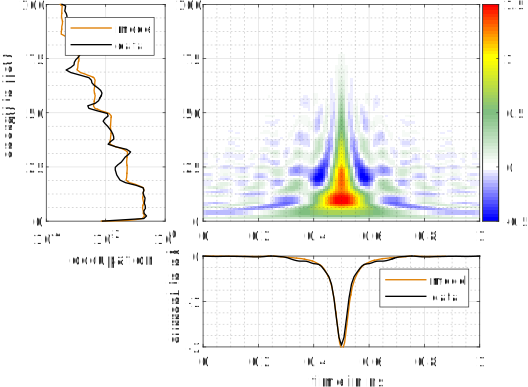
\includegraphics[width = 6.5 cm]{./chap1/wannierwigData_leviton_20ps_1e_51mK_Projected_Gradient_Method-el-0} &
			& 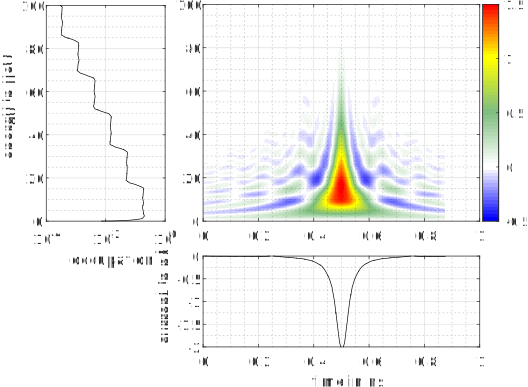
\includegraphics[width = 6.5 cm]{./chap1/wannierwigTheory_leviton_25ps_1e_50mK-el-0} \\
			(c) & & (d) & \\
			& 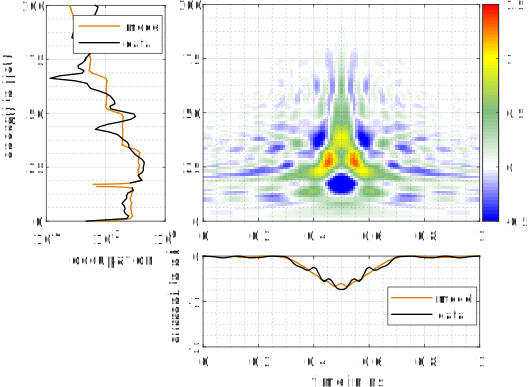
\includegraphics[width = 6.5 cm]{./chap1/wannierwigData_leviton_20ps_1e_51mK_Projected_Gradient_Method-el-1} & &
			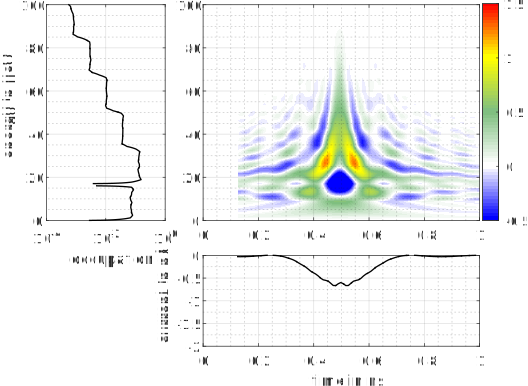
\includegraphics[width = 6.5 cm]{./chap1/wannierwigTheory_leviton_25ps_1e_50mK-el-1} \\
			(e) & & (f) & \\
			& \includegraphics[width = 6.5 cm]{./chap1/wannierwigData_leviton_20ps_1e_51mK_Projected_Gradient_Method-ho-0} & &
			\includegraphics[width = 6.5 cm]{./chap1/wannierwigTheory_leviton_25ps_1e_50mK-ho-0}
		\end{tabular} 
	\end{center}
	\caption{\textbf{Wigner distribution of wavefunctions generated by a twice shorter Lorentzian pulses $\tau = 25$ ps.} \textbf{(a)} Most populated electronic wavefunction numbered 1. It has a strong overlap of 0.96 with the zero temperature theoretical wavefunction. \textbf{(b)} Wavefunction extracted from Wigner distribution calculated numerically. It is a Lorentzian wavefunction of width $\tau = 25$ ps \textbf{(c)} Second most populated electronic wavefunction numbered 2. It differs from the higher energy Lorentzian wavefunction, especially because of its large time spreading. \textbf{(d)}  Second wavefunction extracted from Wigner distribution calculated numerically. \textbf{(e)} Most populated hole wavefunction numbered 1. The energies are below the Fermi level, negative, because it is a hole wavefunction. Its center is shifted by half a period, 0.125 ns, the holes are emitted between electronic wavefunctions. \textbf{(f)} Hole wavefunction extracted from Wigner distribution calculated numerically. It is a Martin-Landauer wavepacket.}
	\label{fig: wannier du 1e 20ps}
\end{figure}

%In figure Fig. \ref{fig: wannier du 1e 20ps}, the wavefunctions measured are plotted.
In the figure Fig. \ref{fig: wannier du 1e 20ps}, we plot the wavefunctions extracted from the Wigner distribution.
In panels (a) and (b) there are the two occupied electronic wavefunctions as in the previous section, and in addition in the panel (c) there is the emitted hole wavefunction.
In the panel (a), even if the marginals look noisier than in previous section, we still have a wavefunction that looks similar to a pure periodic Lorentzian pulse at $T=0$ K.
The current is a Lorentzian peak in the center of the period with a maximum almost twice stronger and a width twice shorter than in the previous section.
The occupation is still linear in a log-lin scale, but it decrease slower with energy and so the steps of width $h\nu$ are less high.
The smaller amplitude of the steps makes them less visible due to measurement noise.
The overlap between this measured wavefunction and a numerically calculated pure periodic Lorentzian pulse of 25 ps width is $0.96$, so they are consistent.
The second electronic state emitted, plotted in figure \ref{fig: wannier du 1e 20ps} (b), does not follow the same trend as the most populated one when the pulse width is divided by 2.
On the contrary its current marginal looks wider than the one in the previous section.
The occupation marginal still presents its maximum at the second $h\nu$ energy step, so there is still a mixed state between the zero temperature Lorentzian wavefunction and a state emitted at higher energy.
This mixed state is also shared with a additional hole wavefunction plotted in panel (c).
For Wigner distribution of holes the energy axis is limited to negative values.
Because the Wigner distribution is non zero only below the Fermi energy chosen here as zero.
The current marginal has also a reverse sign compared to electron, here the current is always positive.
On the current marginal we can remark that its maximum is shifted by half a period of $0.125$ ns compared to both electronic wavefunction.
This is interpreted as the holes are emitted between the electronic wavefunction, thanks to the free space let by shorter pulses.
On the occupation almost only one $h\nu$ step is populated, the higher one in energy.
The thermal excitations emit holes first close to the Fermi level in a Martin-Landauer wavepacket \cite{martin1992wave,roussel2017autopsy} because the occupation equals 1 on the first $h\nu$ step.


\subsection{Two elementary charges Lorentzian pulses}

In last subsections a train of Lorentzian pulses carrying one charge per period is sent and we notice that we emit more than one states. 
In the following we emit on purpose two electrons.
To do so we can generate a train of Lorentzian pulses carrying two charges per period.
The current generated is a train of Lorentzian pulses generated at a repetition rate of 4 GHz, with a width of 40 ps, and an amplitude chosen such that each pulse carries two elementary charge $2e$.

\subsubsection*{Wigner distribution}

\begin{figure}[hpbt]
	\begin{center}
		\begin{tabular}{c c c c}
	
		(a) & & (b) &  \\ 
		& \includegraphics[width = 6cm]{./chap1/wigData_leviton_40ps_2e_51mK_Projected_Gradient_Method}&
		& \includegraphics[width = 6cm]{./chap1/wigTheory_leviton_40ps_2e_50mK}
		\end{tabular} 
	\end{center}
	\caption{\textbf{Wigner distribution of a periodic train of Lorentzian pulses carrying two elementary charges.} \textbf{(a)} The measured current is a Lorentzian pulse carrying 2e.
	One can notice that a pulse carrying twice the charge of the one presented in figure Fig. \ref{fig: wigner du 1e 40ps} results in a Wigner which spreads in a larger energy range.
	The red zone of above one value is still present as in figure Fig. \ref{fig: wigner du 1e 40ps}. 
	%And the pulse in the Wigner distribution is bigger than the first Wigner distribution presented with still a red zone of above one value.
	 \textbf{(b)} Numerical calculation of the Wigner distribution with the same voltage excitation as in panel (a).}
	\label{fig: wigner du 2e 40ps}
\end{figure}

In figure Fig. \ref{fig: wigner du 2e 40ps} is plotted the Wigner distribution measurement result.
The current marginal confirms the Lorentzian shape and the charge $\left|\frac{q}{e}\right| = 1.99$ of the generated current.
On the occupation marginal we remark that the negative energy level are still fully occupied, we do not emit holes by sending an additional electronic charge.
Additionally the Wigner distribution reaches above one value at the pulse location as for the precedent pulses carrying one elementary charge.

\subsubsection*{Emission probabilities and inter-period coherences}

\begin{figure}[hptb]
	\begin{center}
		\begin{tabular}{c c c c}
			
			(a) & & (b) &  \\ 
			& \includegraphics[width = 6.5 cm]{./chap1/JnlData_leviton_40ps_2e_51mK_Projected_Gradient_Method_proba} &
			& \includegraphics[width = 6.5 cm]{./chap1/JnlData_leviton_40ps_2e_51mK_Projected_Gradient_Method_coh} \\
		\end{tabular} 
	\end{center}
	\caption{\textbf{Weights of emission an coherences with a Lorentzian pulse carrying two elementary charges.}\textbf{(a)} Emission probabilities of the main wavefunctions. No holes are emitted, and one electronic wavefunction is emitted at each pulses. \textbf{(b)} Coherences between wavefunctions shifted by $l$ periods. For the wavefunction numbered 1 there is no coherence between periods because it has a probability of 1. For both panels comparaison with calculations at the same temperature is given by light colour with dashed contour symbols and calculations at 0 K with white symbols of dotted contour.}
	\label{fig: Jnl du 2e 40ps}
\end{figure}

In the emission probabilities plotted in figure Fig. \ref{fig: Jnl du 2e 40ps} (a), there are still no holes as seen directly on the Wigner distribution.
The most occupied electron has a probability of $1$.
It is emitted at each period and there are no coherences between different periods as shown by all the blue dots close to 0 in panel (b).
Then there are two other states emitted with probabilities below one.
They are emitted with a probability of $0.67 \pm 0.02$ and $0.26 \pm 0.02$.
The state is a mixed state between two Slater determinant, one between the most populated electron state and the second one generated with a probability $0.67$, and a Slater determinant between the most populated electron state again and the third one obtained with a probability of $0.26$.
For the two last states, as their emission probabilties are not 0 or 1, there are some coherences between periods (see green and red points panel (b)).

\subsubsection*{Wavefunctions}

\begin{figure}[hptb]
	\begin{center}
		\begin{tabular}{c c c c}
			
			(a) & & (b) &  \\ 
			& \includegraphics[width = 6.5 cm]{./chap1/wannierwigData_leviton_40ps_2e_51mK_Projected_Gradient_Method-el-0} &
			& \includegraphics[width = 6.5 cm]{./chap1/wannierwigTheory_leviton_40ps_2e_51mK-el-0} \\
			(c) & & (d) &  \\ 
			& \includegraphics[width = 6.5 cm]{./chap1/wannierwigData_leviton_40ps_2e_51mK_Projected_Gradient_Method-el-1} &
			& \includegraphics[width = 6.5 cm]{./chap1/wannierwigTheory_leviton_40ps_2e_51mK-el-1} \\
			(e) & & & \\
			& \includegraphics[width = 6.5 cm]{./chap1/wannierwigData_leviton_40ps_2e_51mK_Projected_Gradient_Method-el-2} & &
		\end{tabular} 
	\end{center}
	\caption{ \textbf{Wigner distribution of wavefunctions emitted in a two elementary charge pulse.} \textbf{(a)} Wavefunction numbered 1 emitted with unit probability. %Emitted at each period electronic wavefunction numbered 1.  
	The wavefunction is similar to Lorentzian wavefunction but it is too narrow in time. \textbf{(b)} Wavefunction calculated, it is a linear combination of two Lorentzian wavefunction. \textbf{(c)} Second most populated electronic wavefunction numbered 2. This wavefunction is large in time contrary to Lorentzian wavefunction basis. The two most emitted wavefunctions are in fact a linear combination of the Lorentzian wavefunction basis. \textbf{(d)} Second wavefunction obtained from calculation. It is the complemantary linear combination of Lorentzian wavefunction.% in order that it forms a rotation with (b). 
	\textbf{(e)} Third emitted electronic wavefunction numbered 3.}
	\label{fig: wannier du 2e 40ps}
\end{figure}

\begin{figure}[hpbt]
	\centering
	\includegraphics[width = 10cm]{./chap1/dessin_bloch_sphere_data_51mK_v3}
	\caption{\textbf{Bloch sphere representation of couples of Lorentzian pulse basis wavefunctions.} From the two wavefunctions measured we recover the Lorentzian wavefunction basis by linear combination. The results are represented using a analogy with a Bloch sphere. The red point gives the angle coordinate in the equations \eqref{eq: + state rotated}\eqref{eq: - state rotated}. On the axis are plotted the Wigner distributions of the three basis of wavefunctions corresponding to the x, y and z axes.  %is plotted the Wigner distributions of the deduce basis wavefuntions from linear combination of measurements.
	}
	\label{fig: la sphere de bloch de q=2e}
\end{figure}

The three wavefunctions of the three electronic states identified in the above paragraph are plotted in figure Fig. \ref{fig: wannier du 2e 40ps}.
The two first wavefunctions, plotted in panels (a) and (b), do not match the one of the single charge pulse of the same width, in panels (a) and (b) of figure Fig. \ref{fig: wannier el du 1e 40ps}.
The most populated wavefunction in panel (a) does also not match the numerical calculation for a zero temperature single charge Lorentzian pulse.
Its current marginal is thinner than the 40ps width, and its occupation marginal expands on higher energies.
The second wavefunction in panel (b) is also not completely similar to the higher energy Lorentzian state.
Its current marginal has a double peak shape larger than 40 ps.
Its occupation marginal has its two energy $h\nu$ steps almost equal.
If we numerically compute the state of periodic Lorentzian pulses of charge $2e$ at zero temperature, the two electrons state found is a Slater determinant of the two Lorentzian states.
This Slater determinant is the same as the one formed by a couple of any superposition of the two Lorentzian states.
%So it can be the Slater determinant formed by a couple of any superposition of the two Lorentzian states.
All these superpositions can be described by a rotation on the Bloch sphere.
%With the two found superposition states comes from a rotation on a sphere of the initial two Lorentzian state.
If we call $\left|-z\right>$ the low energy initial Lorentzian state, and $\left|+z\right>$ the initial high energy one, we can express any superposition couple $\left|+_{\theta,\phi}\right>$ and $\left|-_{\theta,\phi}\right>$ with equations \eqref{eq: + state rotated} and \eqref{eq: - state rotated}.

\begin{equation}
\left|+_{\theta,\phi}\right> = \cos\left(\frac{\theta}{2}\right)\left|+z\right>+e^{i\phi}\sin\left(\frac{\theta}{2}\right)\left|-z\right> \label{eq: + state rotated}
\end{equation}

\begin{equation}
\left|-_{\theta,\phi}\right> = e^{-i\phi}\sin\left(\frac{\theta}{2}\right)\left|+z\right>-\cos\left(\frac{\theta}{2}\right)\left|-z\right> \label{eq: - state rotated}
\end{equation}

The measured wavefunctions at finite temperature in figure Fig. \ref{fig: wannier du 2e 40ps} (a) and (b) are not the Lorentzian states $\left|-z\right>$, $\left|+z\right>$, but rather a superposition of states obtained from a rotation by angles
%these two rotated by angles 
$\theta = \frac{\pi}{2}\times0.37$ rad and $\phi = 0$ rad.
In figure Fig \ref{fig: la sphere de bloch de q=2e}, we have plotted on a sphere by a red point the angles coordinates of the measured wavefunctions.
On the three axes, x, y and z, we have plotted the wavefunctions deduced from a rotation applied to the measured wavefunctions represented in Fig. \ref{fig: wannier du 2e 40ps}, panels (a) and (c). The wavefunctions $\left|+z\right>$ and $\left|-z\right>$ have a very strong overlap of 0.99 and 0.96 with the theoretical Lorentzian pulses. 
%And on the three axis $x$, $y$, $z$, the wavefunctions couples are deduced by rotation from the measured one in figure Fig. \ref{fig: wannier du 2e 40ps} panel (a) and (c) corresponding to angle coordinates of the red point in figure Fig \ref{fig: la sphere de bloch de q=2e}.
%The wavefunctions $\left|+z\right>$ and $\left|-z\right>$ of figure Fig \ref{fig: la sphere de bloch de q=2e}, deduce from measurement, have very strong overlap $0.99$ and $0.96$, with the theoretical Lorentzian pulses.
The third wavefunction in figure Fig. \ref{fig: wannier du 2e 40ps} (c) is not a Lorentzian pulse as it can be seen on its current marginal.
But it is a higher energy state, as we can see on the occupation marginal and the Wigner distribution, where there is almost no signal in the first $h\nu$ energy step.

\subsection{AC electron and hole Lorentzian pulses}

When sending an electron on a shorter time scale compared to the period, there is also a hole state appearing.
We have also shown in the previous section how we can, on purpose, generate two states of different kind.
Here, we generate in a controlled manner one electron and one hole
%And we have also generate on purpose two electronic states in the previous section.
%We can also generate on purpose two states of different kind, one electron and one hole.
Using the same injection set-up as for other pulses, we send the electron followed by the hole by periodically alternating a Lorentzian pulse with one negative followed by one positive elementary charge.
The Lorentzian pulses are still with an half width at half maximum of 40 ps.
But as the sign of the pulse changes its sign on one pulse other two, the fundamental frequency is divided by 2, and is equal to 2 GHz.
And the harmonics to generate an alternate pulse are only odd number harmonics at 2 GHz, 6 GHz, 10 GHz, ...

\subsubsection*{Wigner distribution}

\begin{figure}[hpbt]
	\begin{center}
		\begin{tabular}{c c c c}
		
		(a) & & (b) &  \\ 
		& \includegraphics[width = 6cm]{./chap1/wigAC_Data_leviton_40ps_1e_JMAP_f_vf} &
		& \includegraphics[width = 6cm]{./chap1/wigTheory_AC_leviton_50ps_1e_60mK}
		
		\end{tabular} 
	\end{center}
	\caption{\textbf{Wigner distribution of a periodic train of alternating electron and hole Lorentzian pulses.} \textbf{(a)} The time scales is twice larger than for above Wigner distribution in order to show the positive and negative Lorentzian current pulse. The two pulses are almost symmetric with red above 1 values in the center of the electronic pulse and blue below 0 values in the center of the hole pulse. \textbf{(b)} Numerical calculations of alternating electron and hole pulse of width $\tau = 50$ ps.}
	\label{fig: wigner du 1e 40ps AC}
\end{figure}

The Wigner distribution measured is represented in figure Fig. \ref{fig: wigner du 1e 40ps AC}.
The time axis range is 0.5 ns twice larger as for previous Wigner distribution because the fundamental frequency is 2 GHz twice smaller than 4 GHz.
The current marginal is, as described in the beginning of this section, in the first half period a negative Lorentzian pulse, in the second half period a positive Lorentzian pulse.
The integral of the current marginal on the first half period or on the second half period, equals one negative or one positive elementary charge.
The occupation marginal has some above 0 values at positive energy, so electron are created.
And symmetrically it has some below 1 values at negative energy, so holes are emitted.
The above zero and below one values spread in energy around the Fermi level on a range of 50 $\upmu$eV, which is bigger than the electronic temperature $T_{\mathrm{elec}} = 50$ mK $= 5$ $\upmu$eV.
The electron and holes are not generated by thermal excitations but by the injected current.
On the Wigner distribution the above 1 values in the electron pulse and the below 0 values in the hole pulse, indicate that the electron and hole states are not classical.


\subsubsection*{Emission probabilities and inter-period coherences}

\begin{figure}[hptb]
	\begin{center}
		\begin{tabular}{c c c c}
			
			(a) & & (b) &  \\ 
			& \includegraphics[width = 5 cm]{./chap1/JnlAC_Data_leviton_40ps_1e_JMAP_f_vf_proba_el} &
			& \includegraphics[width = 5 cm]{./chap1/JnlAC_Data_leviton_40ps_1e_JMAP_f_vf_proba_ho} 
		\end{tabular} 
	\end{center}
	\caption{\textbf{Emission probabilities of the alternating electron and hole Lorentzian pulses.} \textbf{(a)} Probabilities for electronic wavefunctions only. \textbf{(b)} Probabilities for hole wavefunctions only. Same ordering and color code is used for electrons and holes to emphasize the symmetry between electrons and holes. Bars with light colour and dashed contours are numerical calculations at a temperature of $T_{\mathrm{elec}} = 50$ mK. White bars with dotted contours are numerical calculation at $T_{\mathrm{elec}} = 0$ K, even at 0 K there are two wavefunctions emitted of probability $p_{1} = 0.95$ and $p_{2} = 0.05$.}
	\label{fig: pi du 1e 40ps AC}
\end{figure}

In the figure Fig. \ref{fig: pi du 1e 40ps AC} (a) the probabilities for electron wavefunction emission are plotted, and in the panel (b) the probabilities for hole wavefunction emission are plotted.
The two panels (a) and (b) show almost the same results, we emit the same number of electronic and hole states.
As shown in the case of the single electron charge pulse, we emit a mixed state mostly between two states, for the electrons and the holes.

\begin{figure}[hptb]
	\begin{center}
		\begin{tabular}{c c c c}
			
			(a) & & (b) &  \\ 
			& \includegraphics[width = 5 cm]{./chap1/JnlAC_Data_leviton_40ps_1e_JMAP_f_vf_coh_el_el} &
			& \includegraphics[width = 5 cm]{./chap1/JnlAC_Data_leviton_40ps_1e_JMAP_f_vf_coh_ho_ho} \\
			(c) & & &  \\ 
			& \includegraphics[width = 5 cm]{./chap1/JnlAC_Data_leviton_40ps_1e_JMAP_f_vf_coh_el_ho_0} &
			& 
		\end{tabular} 
	\end{center}
	\caption{\textbf{Coherences of the alternating electron and hole Lorentzian pulses.} \textbf{(a)} Coherences between electronic wavefunctions separated by $l$ periods \textbf{(b)} Coherences between hole wavefunctions separated by $l$ periods \textbf{(c)} Coherences between the most populated hole wavefunctions and electronic wavefunctions separated by $l$ periods}
	\label{fig: coh du 1e 40ps AC}
\end{figure}

The figure Fig. \ref{fig: coh du 1e 40ps AC} shows the coherences between states.
In the panel (a) is plotted as before the coherence between two electron wavefunctions translated by $l$ period.
The decrease as a function of $l$ is faster than for the single electron Lorentzian pulse case in \ref{fig: Jnl du 1e 40ps} (b).
It is due to the fact that the fundamental frequency $\nu = 2$ GHz is twice smaller, so the typical number of periods with coherences is $\frac{h\nu}{k_{\mathrm{B}}T} = 2.5$.
The values of coherences are also smaller, because the electronic pulses are more separated with $\nu = 2$ GHz.
They are close to the values of the single electron Lorentzian pulse but multiplying by two the number of period separation $l$.
In the panel (b), we can notice that we have similar results for holes and electrons.
In the panel (c), it is showed that since we emit as many holes as electrons, the coherence between electron and holes are of the same order of magnitude as the coherences between two electrons, or between two holes.
And contrary to the case of the single electron Lorentzian pulse, where at zero temperature all coherences disappear and there is only one wavefunction emitted, in the alternate electron hole pulses, the extra wavefunction and the coherences  are not completely suppressed.


\subsubsection*{Wavefunctions}

\begin{figure}[hptb]
	\begin{center}
		\begin{tabular}{c c c c}
			
			(a) & & (b) &  \\ 
			& \includegraphics[width = 6.5 cm]{./chap1/wannierwigAC_Data_leviton_40ps_1e_JMAP_f_vf-el-0} &
			& \includegraphics[width = 6.5 cm]{./chap1/wannierwigTheory_AC_leviton_50ps_1e_60mK_2GHz-el-0} \\
			(c) & & (d) &  \\ 
			& \includegraphics[width = 6.5 cm]{./chap1/wannierwigAC_Data_leviton_40ps_1e_JMAP_f_vf-el-1} &
			& \includegraphics[width = 6.5 cm]{./chap1/wannierwigTheory_AC_leviton_50ps_1e_60mK_2GHz-el-1} \\
			(e) & & (f) & \\
			& \includegraphics[width = 6.5 cm]{./chap1/wannierwigAC_Data_leviton_40ps_1e_JMAP_f_vf-ho-0} &
			& \includegraphics[width = 6.5 cm]{./chap1/wannierwigAC_Data_leviton_40ps_1e_JMAP_f_vf-ho-1}
		\end{tabular} 
	\end{center}
	\caption{ \textbf{Wavefunctions in both electron and hole pulses represented thanks to Wigner distribution.} \textbf{(a)} Most populated electronic wavefunction numbered 1. \textbf{(b)} Electron wavefunction extracted from the Wigner distribution calculated numerically. \textbf{(c)} Second most populated electronic wavefunction numbered 2. \textbf{(d)} Second electron wavefunction extracted from calculation. It forms with the panel (b) a rotation of the angle $\theta = \frac{\pi}{2}\times 0.36$ from the Lorentzian wavefunctions. \textbf{(e)} Most populated hole wavefunction numbered 1. \textbf{(f)} Second most populated hole wavefunction numbered 2. These wavefunctions are similar to the one obtained for the Lorentzian pulse carrying two elementary excitations. They are linear combinations of the Lorentzian wavefunction basis.}
	\label{fig: wannier du 1e 40ps AC}
\end{figure}

Thanks to emission probabilities, we can focus on four wavefunctions plotted in the figure Fig. \ref{fig: wannier du 1e 40ps AC}.
Two of them are electron states in panels (a) and (c), with (a) the most likely electron state.
And the last two in panels (e) and (f) are hole states, with (e) the most emitted hole state.
The hole Wigner distribution (e) and (f) are almost identical to their respective electron Wigner distribution (a) and (c), with the differences that energy axis have opposite signs and the time axis is translated by $0.25$ ns.
The opposite signs express the difference between electron defined as the creation of a charge above the Fermi level, and holes defined as the removal of a charge below the Fermi level.
The time translation of $0.25$ ns is equal to a half-period, so the electron states are centred at the negative charge pulse and the holes at the positive charge pulse.
The couples of electronic states emitted in panels (a) and (b) looks like the two wavefunctions of the two elementary charge per pulse in Fig. \ref{fig: wannier du 2e 40ps} (a) and (c).
Their difference is their energy steps in the occupation marginals which are twice smaller since $h\nu$ is twice smaller here.
Still the two emitted wavefunction are not the zero temperature single charge Lorentzian states as in the figure Fig. \ref{fig: wannier el du 1e 40ps} (b) and (d).
They are, like the double charge Lorentzian, a superposition of these two defined by equations \eqref{eq: + state rotated} \eqref{eq: - state rotated} with an angle $\theta = \frac{\pi}{2}\times 0.36$ and $\phi = 0$.
After rotation the overlaps between $\left|+z\right>$ and $\left|-z\right>$ and the zero temperature single charge Lorentzian states are of $0.97$ and $0.95$ compared to $0.89$ and $0.91$ before rotation.
This effect is also observed for numerical calculations in the figure Fig. \ref{fig: wannier du 1e 40ps AC} panel (b) and (d), which have an overlap of $0.97$ and $0.94$ after rotation compared to $0.84$ and $0.86$ before rotation.



